\chapter{Evaluation protocol and experimental results}
\label{cap:sperimentale}

The performance of a model also depends on the way the evaluation is carried out. The division of the subjects, the normalisation of the features, the handling of the imbalance and the choice of the decision threshold can change the result even when the classifier is left unchanged.

This chapter will be used to analyse two fundamental aspects:
in the first part of the chapter we shall define the protocol used to make the experiments comparable, while in the second part we shall analyse the effect of the representation, of the architecture and of the main parameters of the pipeline. Finally we shall verify what happens when the definition of the task, the viewpoint of the camera and the dataset change.

\section{Experimental protocol}
\label{cap:protocollo}

In the comparisons that follow, metric, subject partition, normalisation and decision threshold were kept fixed. Not all the choices made during the development are, however, entirely independent of the data used in the evaluation. In particular, the threshold of $0{,}50$ was adopted after an exploratory comparison between several rules, while feature selection and the parameter $K$ also used information coming from subjects subsequently employed in the test. These cases are declared and checked separately in Section~\ref{sec:misura_leakage}.

\subsection{Class imbalance and metrics}
\label{sec:metriche}

The subset of UP-Fall used for the evaluation comprises 58.359 frames from Camera~1, distributed over 110 recordings and ten subjects. The pose is available in 92,3\% of the frames. The distribution of the labels is reported in Table~\ref{tab:etichette_valutazione}.

\begin{table}[ht]
\centering
\caption{Distribution of the frame-level labels in the subset
of UP-Fall used for the evaluation.}
\label{tab:etichette_valutazione}
\begin{tabular}{cccc}
\toprule
\textbf{Label} & \textbf{Meaning} &
\textbf{Frames} & \textbf{Share} \\
\midrule
0 & ordinary activity / preceding phase & 50.264 & 86,1\% \\
1 & fall transition & 2.771 & 4,7\% \\
2 & post-fall state & 5.324 & 9,1\% \\
\bottomrule
\end{tabular}
\end{table}

After the temporal windows have been built, 11.719 sequences are obtained, of which 1.491 are positive, that is 12,72\%. Across the different subjects, the number of positive windows in the test ranges from 104 to 171. The dataset is therefore imbalanced towards the negative class. A classifier that assigned every window to the negative class would reach about 87,3\% accuracy without recognising a single fall. This is why accuracy is not used as the main metric.

In order to evaluate the classifier, precision and recall were considered separately. Denoting by $TP$ the true positives, by $FP$ the false positives and by $FN$ the false negatives, the two metrics are defined as
\[
\mathrm{precision}
=
\frac{TP}{TP+FP},
\]

\[
\mathrm{recall}
=
\frac{TP}{TP+FN}.
\]

Precision measures how many of the windows flagged are actually positive, while recall measures how many positive windows are recognised.
Since in fall detection greater weight has to be given to false negatives, without ignoring false positives, the summary measure used is

\[
F_\beta =
(1+\beta^2)
\frac{\mathrm{precision}\cdot\mathrm{recall}}
     {\beta^2\,\mathrm{precision}+\mathrm{recall}},
\]
with
\[
\beta=2.
\]

$F_2$ therefore assigns greater weight to recall. The value of $\beta$ was fixed before the comparison between the models. Recall, false negatives and false positives are nonetheless also reported in the results, because configurations with similar values of $F_2$ may produce different errors.

The imbalance is also handled during training. For every fold the classes are assigned weights inversely proportional to their frequency, computed on the training data alone.
Subsampling of the negative class was not used. With 1.491 positive windows out of 11.719, full balancing would require removing about 85,4\% of the negative windows, and with them a large part of the daily activities available.

\subsection{LOSO partitioning}
\label{sec:loso}

In the dataset every subject appears in several recordings, from which many temporal windows are derived, often very similar to one another.
In the earliest trials the split was made at recording level. The recordings were therefore separated between training and test, but the same subject could appear in both sets.

This split cannot assess the behaviour of the system on a person never observed. A \emph{Leave-One-Subject-Out} validation was therefore adopted. The subset used comprises ten subjects and, for every fold, one subject is used for the test, one for validation and the other eight for training. The validation subject is the one following the test subject in a circular order, so that the rule always remains the same. The composition of the ten folds, together with the number of windows used for training and the positive ones present in the test, is reported in Table~\ref{tab:fold}.

\begin{table}[ht]
\centering
\caption{Composition of the ten folds used in the LOSO validation.}
\label{tab:fold}
\resizebox{\textwidth}{!}{%
\begin{tabular}{cccc}
\toprule
\textbf{Test subject} &
\textbf{Validation} &
\textbf{Training windows} &
\textbf{Positive in the test} \\
\midrule
Subject\_01 & Subject\_02 & 9.318 & 129 \\
Subject\_02 & Subject\_03 & 9.320 & 157 \\
Subject\_03 & Subject\_04 & 9.327 & 165 \\
Subject\_04 & Subject\_05 & 9.589 & 104 \\
Subject\_05 & Subject\_06 & 9.734 & 144 \\
Subject\_06 & Subject\_07 & 9.446 & 135 \\
Subject\_07 & Subject\_08 & 9.225 & 168 \\
Subject\_08 & Subject\_09 & 9.221 & 168 \\
Subject\_09 & Subject\_10 & 9.272 & 171 \\
Subject\_10 & Subject\_01 & 9.300 & 150 \\
\bottomrule
\end{tabular}
}
\end{table}

Every configuration is therefore trained ten times and evaluated each time on a subject never used during training and validation. This avoids having recordings or windows belonging to the same person present in the training and in the test at the same time. The protocol also brings out the variability between people. Across the different experiments the standard deviation of $F_2$ generally lies between about 0,05 and 0,14. For this reason the differences between configurations are always compared with the dispersion between subjects.

When two configurations are evaluated on the same ten subjects, a paired fold-by-fold comparison is moreover carried out, so as to understand whether the differences are present in a similar way across the various subjects, or whether the mean value depends above all on a few cases.

\subsection{Feature normalisation}
\label{sec:normalizzazione}

The features used comprise angles, velocities, geometric ratios and integral quantities, and can therefore have very different scales. In the first checks, the ratio between the standard deviation of the feature with the largest scale and that of the feature with the smallest reached 646, with the risk of giving greater weight to the features with higher numerical variability. For every feature the standardisation

\[
z_j =
\frac{x_j-\mu_j}{\sigma_j}.
\]

was therefore applied.

Mean and standard deviation are computed separately in each fold using only the training data, and are then applied unchanged to validation and test. The statistics are computed on the frames before the windows are built. With windows of 22 samples and a stride of 2, two consecutive windows share 20 samples. Computing the statistics after the windowing would mean counting the same data several times.

For fourteen features with strongly skewed distributions the transformation
\[
x' = \operatorname{sgn}(x)\log(1+|x|),
\]

is moreover applied first.

The features concerned are the nine integral quantities, the angular velocity of the trunk, the velocity of the head, the velocity of the hips, the velocity of the head with respect to the hips and the normalised width of the body. The list was defined by observing the distributions and not through an automatic criterion.
After these operations the ratio between the scales dropped from 646 to values lying roughly between 1,05 and 1,35. The parameters of the transformation are saved together with the model and reused during inference.

\subsection{Choice of the decision threshold}
\label{sec:soglia}

For every temporal window the classifier produces a score $p$. In order to establish whether a window corresponds to a fall, the decision is obtained by comparing it with a threshold $\theta$:

\[
\hat{y} =
\begin{cases}
1, & p \geq \theta,\\
0, & p < \theta.
\end{cases}
\]

A lower threshold tends to increase recall, but also the number of false positives. A higher threshold instead makes the classifier more selective.
In the earliest trials the threshold was not handled uniformly and was in some cases changed by hand. In order to make the configurations comparable, a procedure was therefore tested that chose, for every fold, the threshold maximising $F_2$ on the validation subject, and then applied that value to the test subject. The thresholds obtained across the ten folds are:

\[
0{,}01,\;
0{,}02,\;
0{,}22,\;
0{,}43,\;
0{,}71,\;
0{,}75,\;
0{,}90,\;
0{,}94,\;
0{,}95,\;
0{,}99,
\]

The standard deviation is about 0,37. A threshold chosen on a single validation subject therefore turns out to be unstable: a threshold suited to that person is not necessarily suited to the test subject as well. Six rules were therefore compared, applied to the same scores already produced by the ten folds.

\begin{table}[ht]
\centering
\caption{Comparison between the six rules used to choose the threshold.}
\label{tab:soglie}
\resizebox{\textwidth}{!}{%
\begin{tabular}{lccc}
\toprule
\textbf{Rule} &
\textbf{mean $F_2$ $\pm$ dev.} &
\textbf{Recall} &
\textbf{mean threshold $\pm$ dev.} \\
\midrule
Maximum $F_2$ on the validation set
    & 0{,}810 $\pm$ 0{,}117 & 0{,}908 & 0{,}59 $\pm$ 0{,}37 \\
Maximum $F_1$
    & 0{,}790 $\pm$ 0{,}120 & 0{,}851 & 0{,}70 $\pm$ 0{,}34 \\
Youden index
    & 0{,}808 $\pm$ 0{,}117 & 0{,}910 & 0{,}59 $\pm$ 0{,}37 \\
Prevalence
    & 0{,}787 $\pm$ 0{,}116 & 0{,}858 & 0{,}68 $\pm$ 0{,}35 \\
Increased prevalence
    & 0{,}823 $\pm$ 0{,}136 & 0{,}972 & 0{,}43 $\pm$ 0{,}31 \\
Fixed threshold $\theta=0{,}50$
    & 0{,}851 $\pm$ 0{,}078 & 0{,}926 & 0{,}50 $\pm$ 0{,}00 \\
\bottomrule
\end{tabular}
}
\end{table}

In this comparison the fixed threshold of $0{,}50$ produces the highest mean value of $F_2$ and a lower dispersion than the rules that depend on the validation subject.

For the subsequent experiments $\theta=0{,}50$ is therefore used for all the folds and all the configurations. It must, however, be made clear that the choice of 0,50 came after the comparison of the six rules on the test folds. It cannot therefore be regarded as a threshold chosen independently of the results. Once adopted, however, it is no longer recomputed on the validation or test subjects and remains the same in all the comparisons that follow.
The only exception is the \emph{oracle} threshold used in the transfer to UR-Fall. In that case the threshold is computed using the labels of the target dataset, exclusively for a diagnostic analysis.

\section{Joint effect of the protocol corrections}
\label{sec:baseline}

Before the corrections, the classifier recognised no positive example and produced $F_1=0$. Analysing the pipeline, three problems were identified: a coherent normalisation was missing, the data were split by recording rather than by subject, and some choices also used data subsequently employed in the verification. Normalisation and partitioning were corrected, while the data-dependent choices are discussed further on.

\begin{table}[ht]
\centering
\caption{Joint effect of the main corrections introduced in the protocol.}
\label{tab:correzioni}
\resizebox{\textwidth}{!}{%
\begin{tabular}{lcc}
\toprule
 & \textbf{Initial configuration} &
   \textbf{Subsequent configuration} \\
\midrule
$F_1$ & 0,000 & 0,234 \\
True positives & 0 & 144 \\
Maximum ratio between the scales & 646$\times$ & 1,05--1,35$\times$ \\
Subjects shared between training and test & 5 out of 5 & 0 \\
\bottomrule
\end{tabular}
}
\end{table}

Table~\ref{tab:correzioni} reports $F_1$ and not $F_2$ because it is the only measure recorded for the initial configuration, which predates the choice of the metric used in the subsequent experiments. The value must therefore not be compared directly with the values of $F_2$ reported in the rest of the chapter.

After the corrections, the number of true positives went from 0 to 144 and $F_1$ reaches 0,234. The improvement cannot be attributed to a single change, because the corrections were introduced together. The comparison does show, however, that the initial failure did not depend on the architecture of the classifier alone.

\section{Comparison between representations and architectures}
\label{sec:grandezze}

Two elements of the pipeline were checked separately: the representation of the movement supplied to the classifier, and the architecture used to process it. In both cases the rest of the protocol is kept unchanged.

\subsection{Comparison between representations}
\label{sec:featureset}

The first experiment concerns the representation of the movement supplied to the classifier. The geometric representations A1, A2 and A3, described in Chapter~\ref{cap:metodologia}, were initially compared in the five-subject experimental configuration.

\begin{table}[ht]
\centering
\caption{Preliminary comparison between the three geometric representations on five subjects.}
\label{tab:rappresentazioni5}
\begin{tabular}{lcc}
\toprule
\textbf{Representation} & \textbf{$F_2$} & \textbf{Recall} \\
\midrule
A1 --- image plane & $0{,}834 \pm 0{,}121$ & -- \\
A2 --- 3D world landmarks & $0{,}867 \pm 0{,}099$ & -- \\
A3 --- body-centred frame & $0{,}857 \pm 0{,}088$ & 0,929 \\
\bottomrule
\end{tabular}
\end{table}

A2 reaches the highest mean value of $F_2$, but between the largest and the smallest value there are only 0,033 points, against standard deviations lying between 0,088 and 0,121. In this first trial the differences therefore turn out to be small with respect to the variability between subjects.

This comparison moreover presents a problem identified later in the A2 features. Two quantities used the translation of the hips in the \emph{world landmarks}. MediaPipe, however, places the hips at the origin of its own reference system, and their translation is almost nil.
Over forty consecutive frames, for example, the standard deviation of the position of the hips is $3\cdot10^{-5}$ metres, against $1{,}75\cdot10^{-2}$ metres for the nose. The two features were therefore measuring mainly numerical noise and were removed.

For the same reason, in the integral quantities of A2 the movement is followed using the nose instead of the hips. Table~\ref{tab:rappresentazioni5} must therefore be read as a preliminary comparison, predating this correction. After the change, the comparison was repeated on ten subjects, using the Random Forest with 50 trees, Camera~1, the LOSO protocol and the fixed threshold $\theta=0{,}50$.

\begin{table}[htbp]
\centering
\caption{Comparison between three feature configurations on ten subjects. Random Forest with 50 trees, Camera~1, LOSO protocol and threshold $0{,}50$.} \label{tab:rappresentazioni10}
\begin{tabular}{lcc}
\toprule
\textbf{Configuration} & \textbf{$F_2$} & \textbf{Recall} \\
\midrule
A3 without integral quantities (10) & $0{,}831 \pm 0{,}117$ & 0,884 \\
A3 with integral quantities (13) & $0{,}832 \pm 0{,}119$ & 0,881 \\
Subset selected by DTW (12) & $0{,}825 \pm 0{,}080$ & 0,849 \\ \bottomrule
\end{tabular}
\end{table}

The differences between the three configurations are small. The mean value of $F_2$ ranges from $0{,}825$ to $0{,}832$, an overall spread of $0{,}007$, while the standard deviation reaches $0{,}119$. Adding the three integral quantities, at equal $h_{\text{pav}}$, changes the mean value by a mere $+0{,}001$. The subset selected by DTW shows instead a variation of $-0{,}007$ with respect to complete A3. This comparison does not, however, measure the effect of the selection alone, because the DTW subset does not contain $h_{\text{pav}}$, which is present in the other two configurations. The difference observed therefore reflects both effects.

With the sample size available we therefore observe no difference in performance on UP-Fall attributable to the addition of the integral quantities or to the DTW selection. The effect of these representations is checked again in the experiments on transfer to conditions different from the benchmark.

\subsection{Comparison between architectures}
\label{sec:architetture}

In order to assess the effect of the architecture, representation, windows, LOSO folds, normalisation and threshold were kept fixed.
The only element that changes is therefore the classifier. The structure of the models and their parameters are described in Chapter~\ref{cap:metodologia}.
Six architectures were compared: LSTM, GRU, 1D CNN,
Transformer, a graph network and a Random Forest used as a non-sequential reference.

\begin{table}[ht]
\centering
\caption{Comparison between the six architectures using the same
LOSO protocol on ten subjects.}
\label{tab:architetture}
\begin{tabular}{lccccr}
\toprule
\textbf{Model} &
\textbf{$F_2$} &
\textbf{Recall} &
\textbf{FN} &
\textbf{FP} &
\textbf{Model size} \\
\midrule
GRU & $0{,}857 \pm 0{,}089$ & 0,940 & 89 & 938 & 24.483 \\ 1D CNN & $0{,}838 \pm 0{,}100$ & 0,938 & 93 & 1.134 & 46.147 \\ Transformer & $0{,}837 \pm 0{,}082$ & 0,920 & 119 & 969 & 34.499 \\ LSTM & $0{,}829 \pm 0{,}084$ & 0,945 & 82 & 1.266 & 32.227 \\ Random Forest & $0{,}825 \pm 0{,}076$ & 0,844 & 232 & 468 & 12.928 nodes \\ Graph & $0{,}794 \pm 0{,}087$ & 0,860 & 209 & 934 & 12.323 \\
\bottomrule
\end{tabular}
\end{table}

The GRU obtains the highest mean value of $F_2$, 0,857, followed by the 1D CNN with 0,838 and the Transformer with 0,837. Leaving the graph network aside, the difference between the largest and the smallest value is 0,032, against a standard deviation for the GRU of 0,089.

The errors, however, behave differently. The LSTM has the highest recall, 0,945, and 82 false negatives, but produces 1.266 false positives, against the 938 of the GRU. The Random Forest is instead more selective: its mean $F_2$ is 0,825 and recall drops to 0,844, with 232 false negatives, but it produces only 468 false positives, about half as many as the GRU and little more than a third of the LSTM.

\begin{figure}[htbp]
\centering
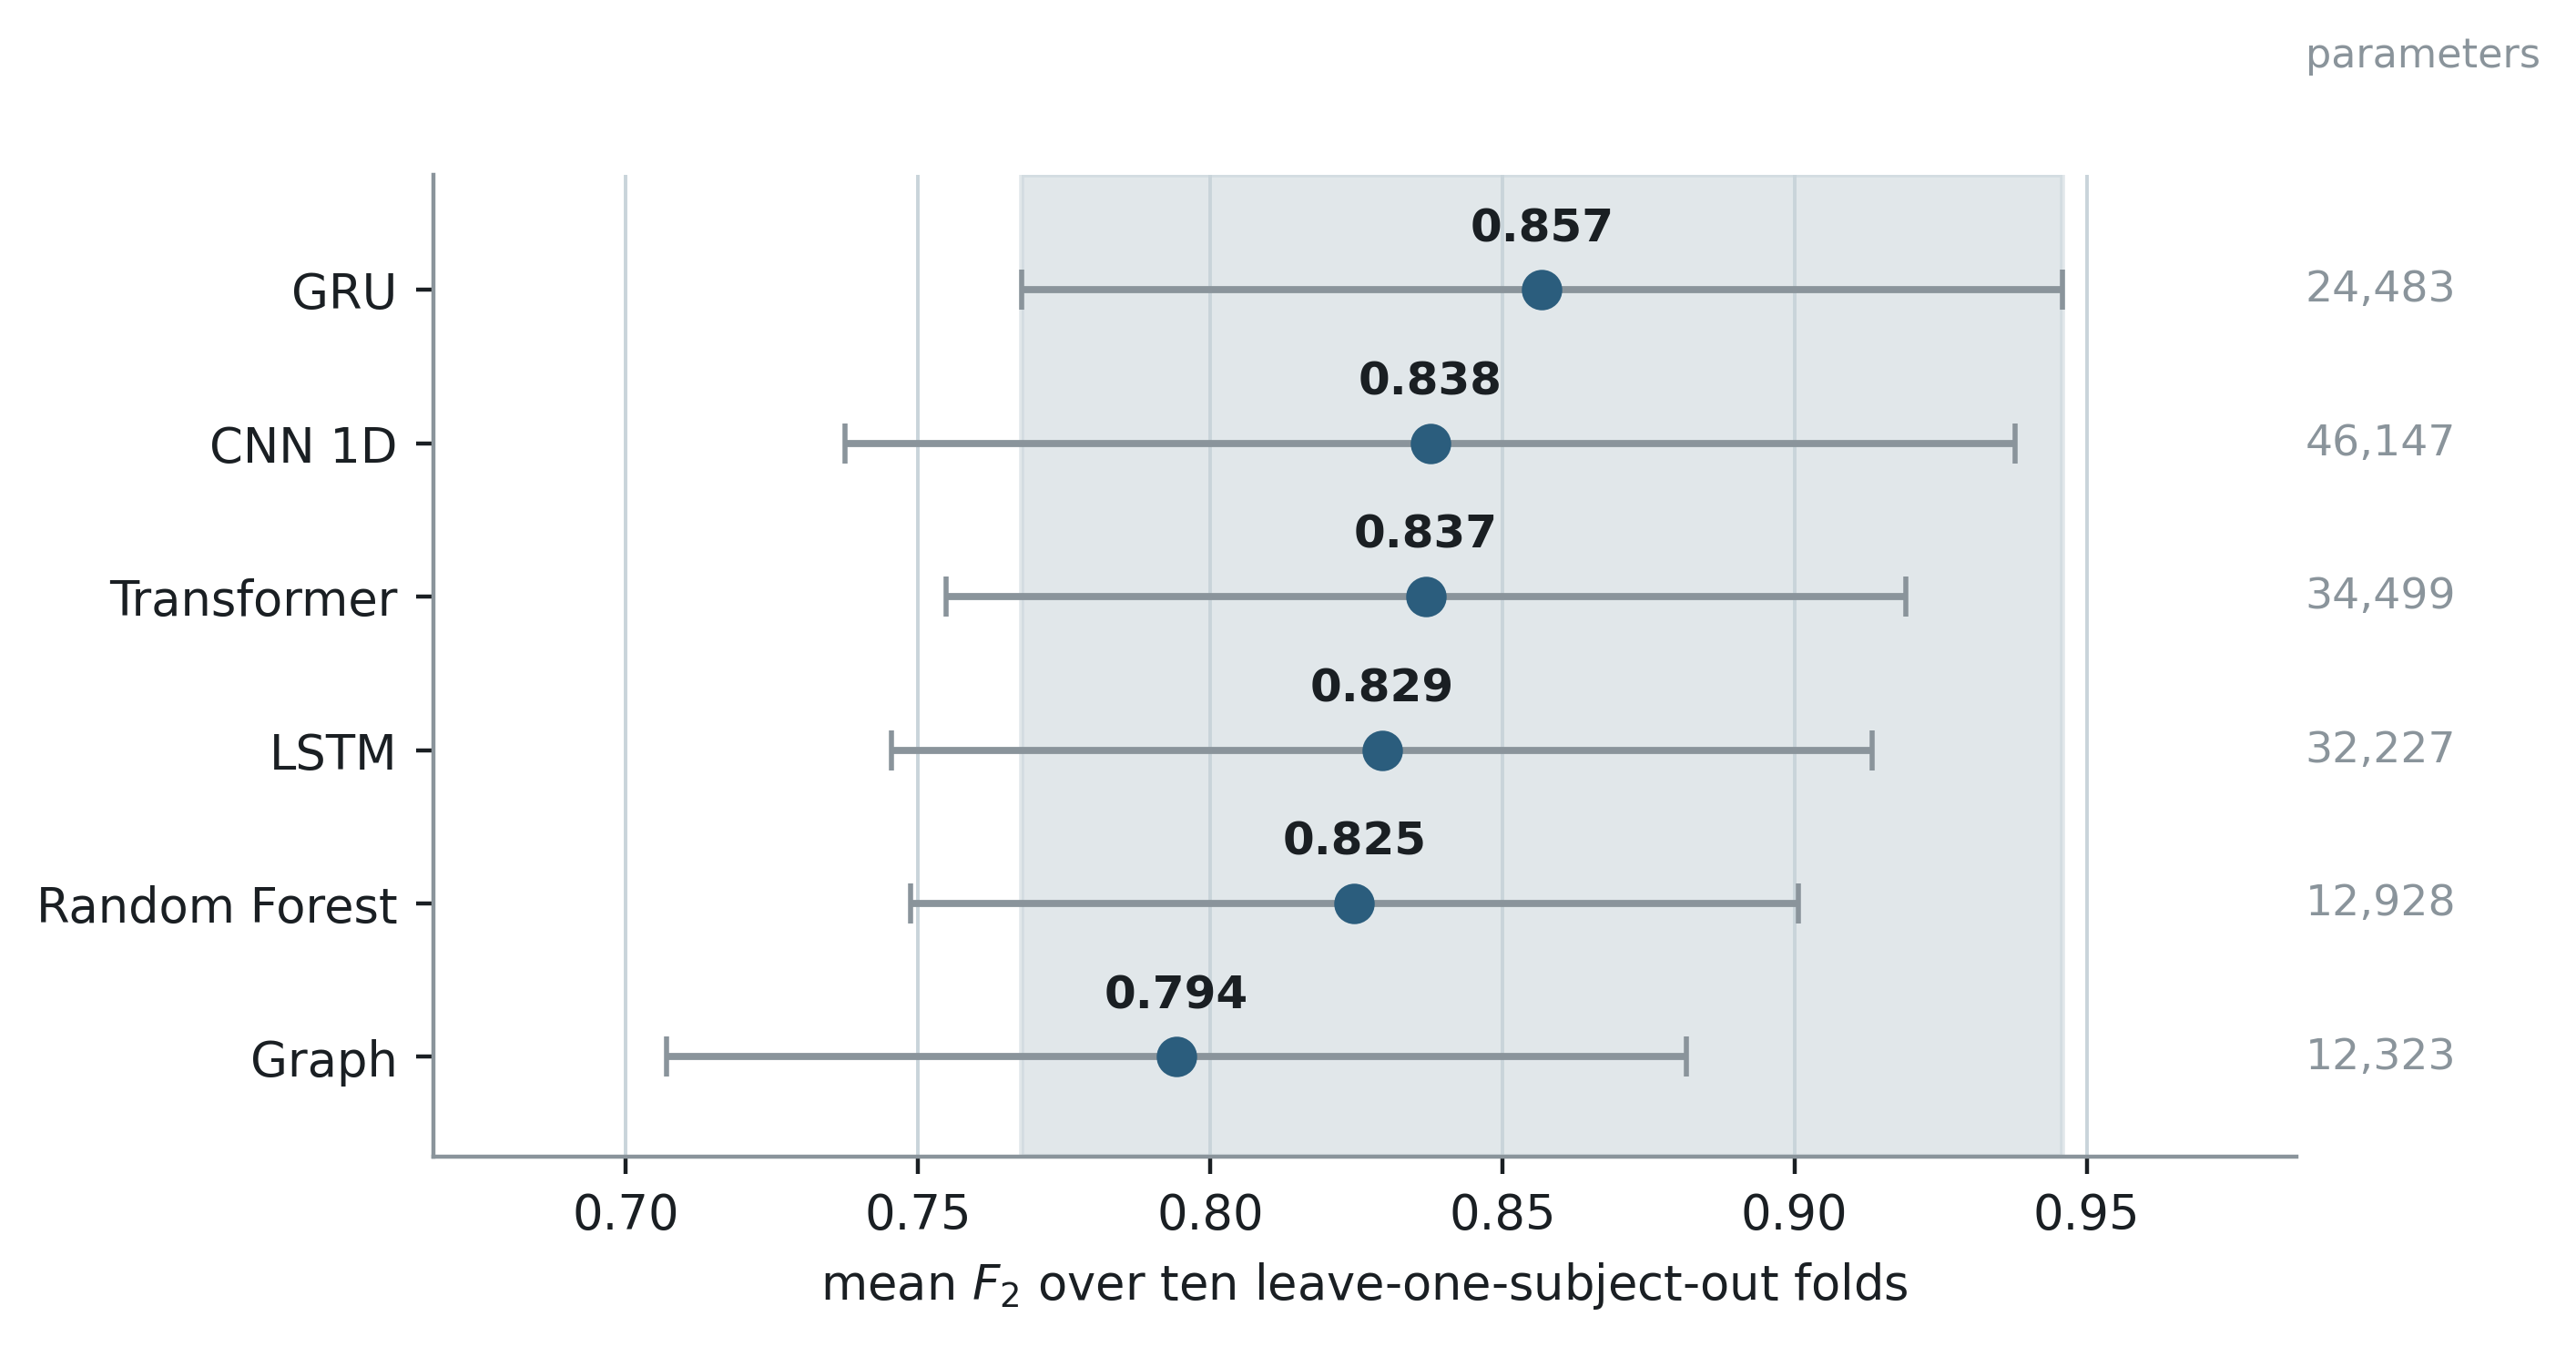
\includegraphics[width=\textwidth]{figure/fig_architetture_en.png}
\caption{Comparison between the six architectures. The error bars represent the dispersion across the ten subjects.}
\label{fig:architetture}
\end{figure}

\begin{figure}[htbp]
\centering
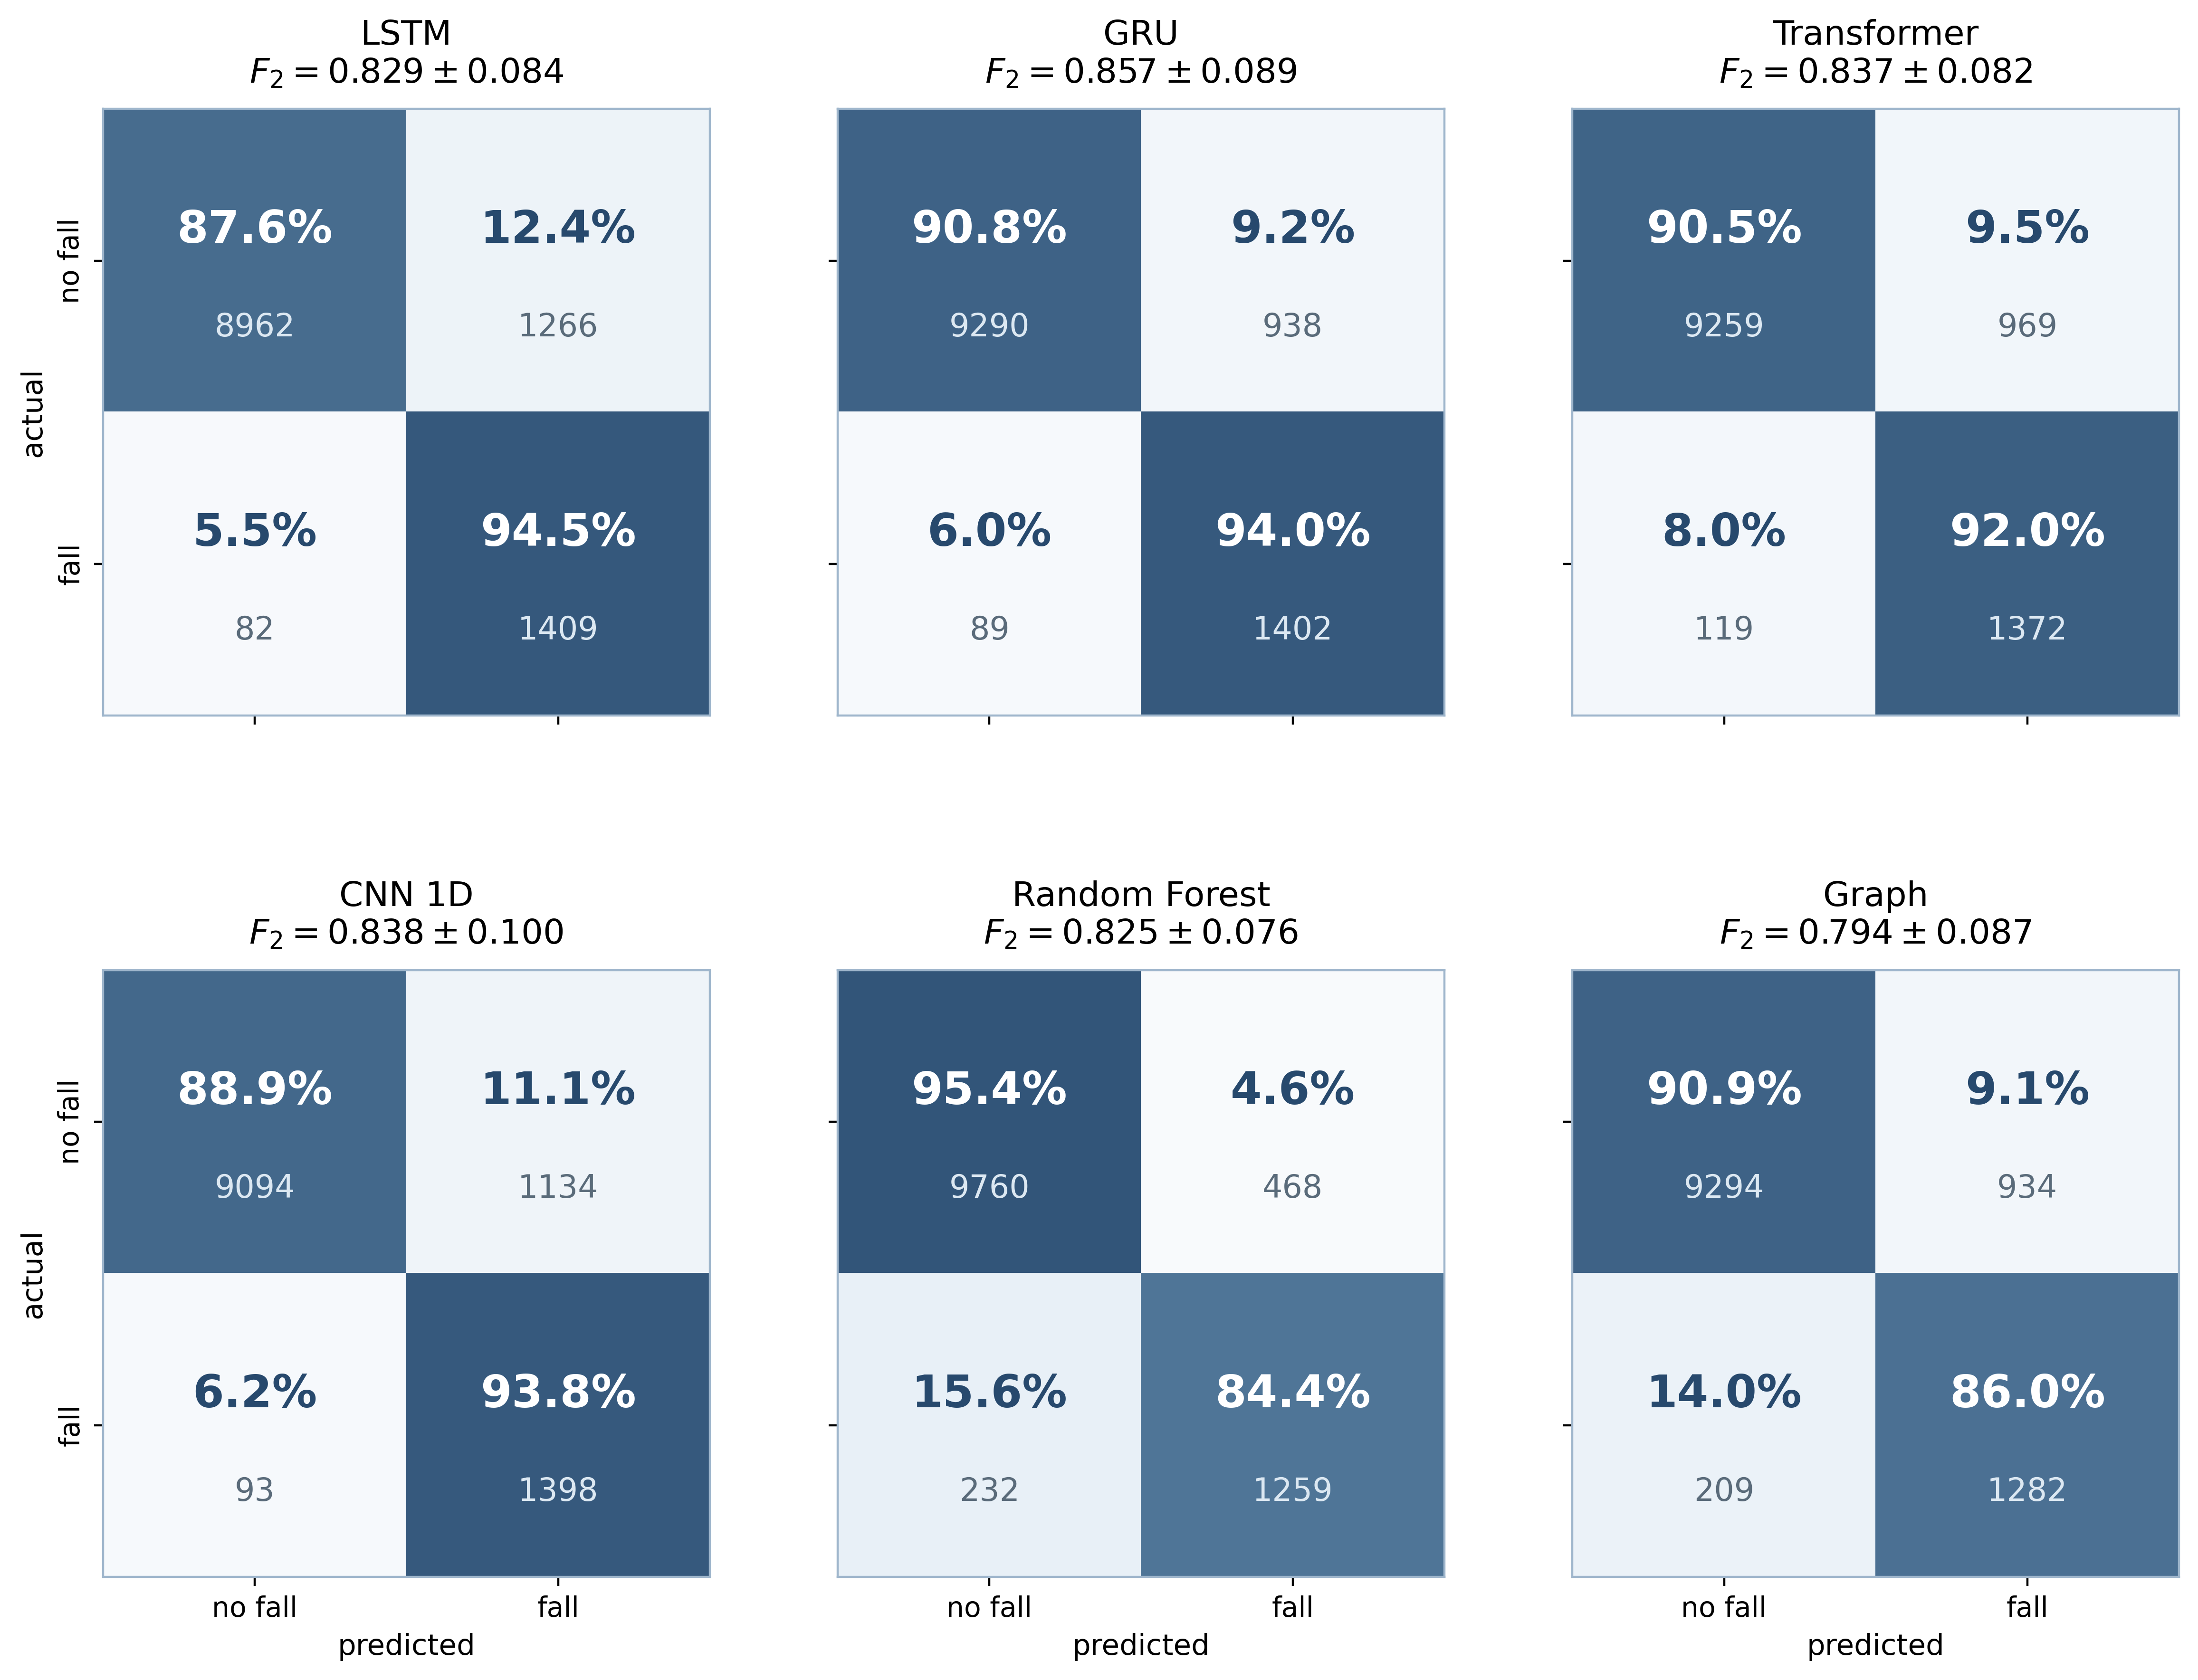
\includegraphics[width=0.85\textwidth]{figure/fig_confusione_en.png}
\caption{Confusion matrices of the six architectures, obtained by pooling the ten verification folds.}
\label{fig:confusione}
\end{figure}

The graph network reaches $F_2=0{,}794\pm0{,}087$. In this implementation the nodes represent the twelve features supplied to the classifier and not the body joints directly. The result therefore concerns this specific configuration and not graph networks applied to the skeleton in general.
The number of parameters shows no evident relationship with performance. The 1D CNN is the neural model with the largest number of parameters, but it does not reach the highest value of $F_2$. The GRU, by contrast, uses about 24\% fewer parameters than the LSTM while obtaining a higher $F_2$.

In order to check the differences on the individual subjects, the models were also compared fold by fold using the GRU as reference. The values obtained are $t=-1{,}16$ for the 1D CNN, $t=-1{,}22$ for the Transformer and $t=-1{,}24$ for the Random Forest. The LSTM and the graph network instead produce $t=-2{,}98$ and $t=-3{,}14$ respectively. Taking into account the five comparisons made against the GRU, however, the critical value corrected for multiple comparisons rises to about 3,25, and no difference exceeds it.

With the number of subjects available we therefore measure no clear difference between the main architectures considered. The architectures were not subjected to a systematic hyperparameter search. The comparison therefore concerns the configurations actually used, and not the respective families of models in general.

\subsection{Analysis of the differences and sample size}

The preceding configurations were evaluated on the same subjects. It is therefore possible to compare the results fold by fold and to use the variability observed in order to estimate how many subjects would be needed to detect the differences measured. Table~\ref{tab:numerosita} reports the mean difference, the value of the paired $t$ test and an estimate of the sample size required with $\alpha=0{,}05$ and 80\% power.

\begin{table}[htbp]
\centering
\caption{Sample size estimated in order to detect some of the differences observed.
The estimate uses a two-tailed paired $t$ test, with $\alpha=0{,}05$ and
80\% power.}
\label{tab:numerosita}
\begin{tabular}{lccc}
\toprule
\textbf{Comparison} &
\textbf{Difference} &
\textbf{$t$} &
\textbf{Subjects required} \\
\midrule
Window of 44 instead of 22 & $+0{,}091$ & $+3{,}62$ & 6 \\
GRU vs graph network & $-0{,}063$ & $-3{,}14$ & 8 \\
GRU vs LSTM & $-0{,}027$ & $-2{,}98$ & 9 \\
GRU vs Random Forest & $-0{,}032$ & $-1{,}24$ & 52 \\
GRU vs Transformer & $-0{,}020$ & $-1{,}22$ & 54 \\
GRU vs 1D CNN & $-0{,}019$ & $-1{,}16$ & 58 \\
DTW selection instead of all of A3 & $-0{,}007$ & $-0{,}21$ & 1.833 \\
Integral quantities added to A3 & $+0{,}001$ & $+0{,}18$ & 2.373 \\
\bottomrule
\end{tabular}
\end{table}

Between the GRU and the Random Forest the mean difference is 0,032, but it varies considerably across subjects and the estimated sample size rises to 52. Between the GRU and the LSTM the gap is slightly smaller, 0,027, but more consistent across the folds, and the estimate drops to nine subjects. The differences introduced by the DTW selection and by the integral quantities are instead very small with respect to the variability between subjects.

The length of the window and some definitions of the task, by contrast, produce more evident effects. Going from 22 to 44 samples increases the mean $F_2$ by 0,091, with $t=3{,}62$, and is therefore detectable even with the number of subjects available.

\section{Sensitivity analysis}
\label{sec:sensibilita}

Besides the main choices, some parameters of the pipeline were analysed while the rest of the configuration was kept unchanged: number of trees of the Random Forest, sampling frequency, window length, availability of the landmarks and noise in the coordinates. The aim is not to find the optimal value of every parameter, but to verify how far performance depends on the choices adopted.

\subsection{Model size}
\label{sec:dimensione}

The first analysis concerns the number of trees of the Random Forest. The configuration used in the pipeline employs 50 trees, a value inherited from the initial prototype and not chosen through an experimental search. Six configurations between 10 and 400 trees were therefore compared, keeping data, features and evaluation protocol unchanged.

\begin{figure}[ht]
    \centering
    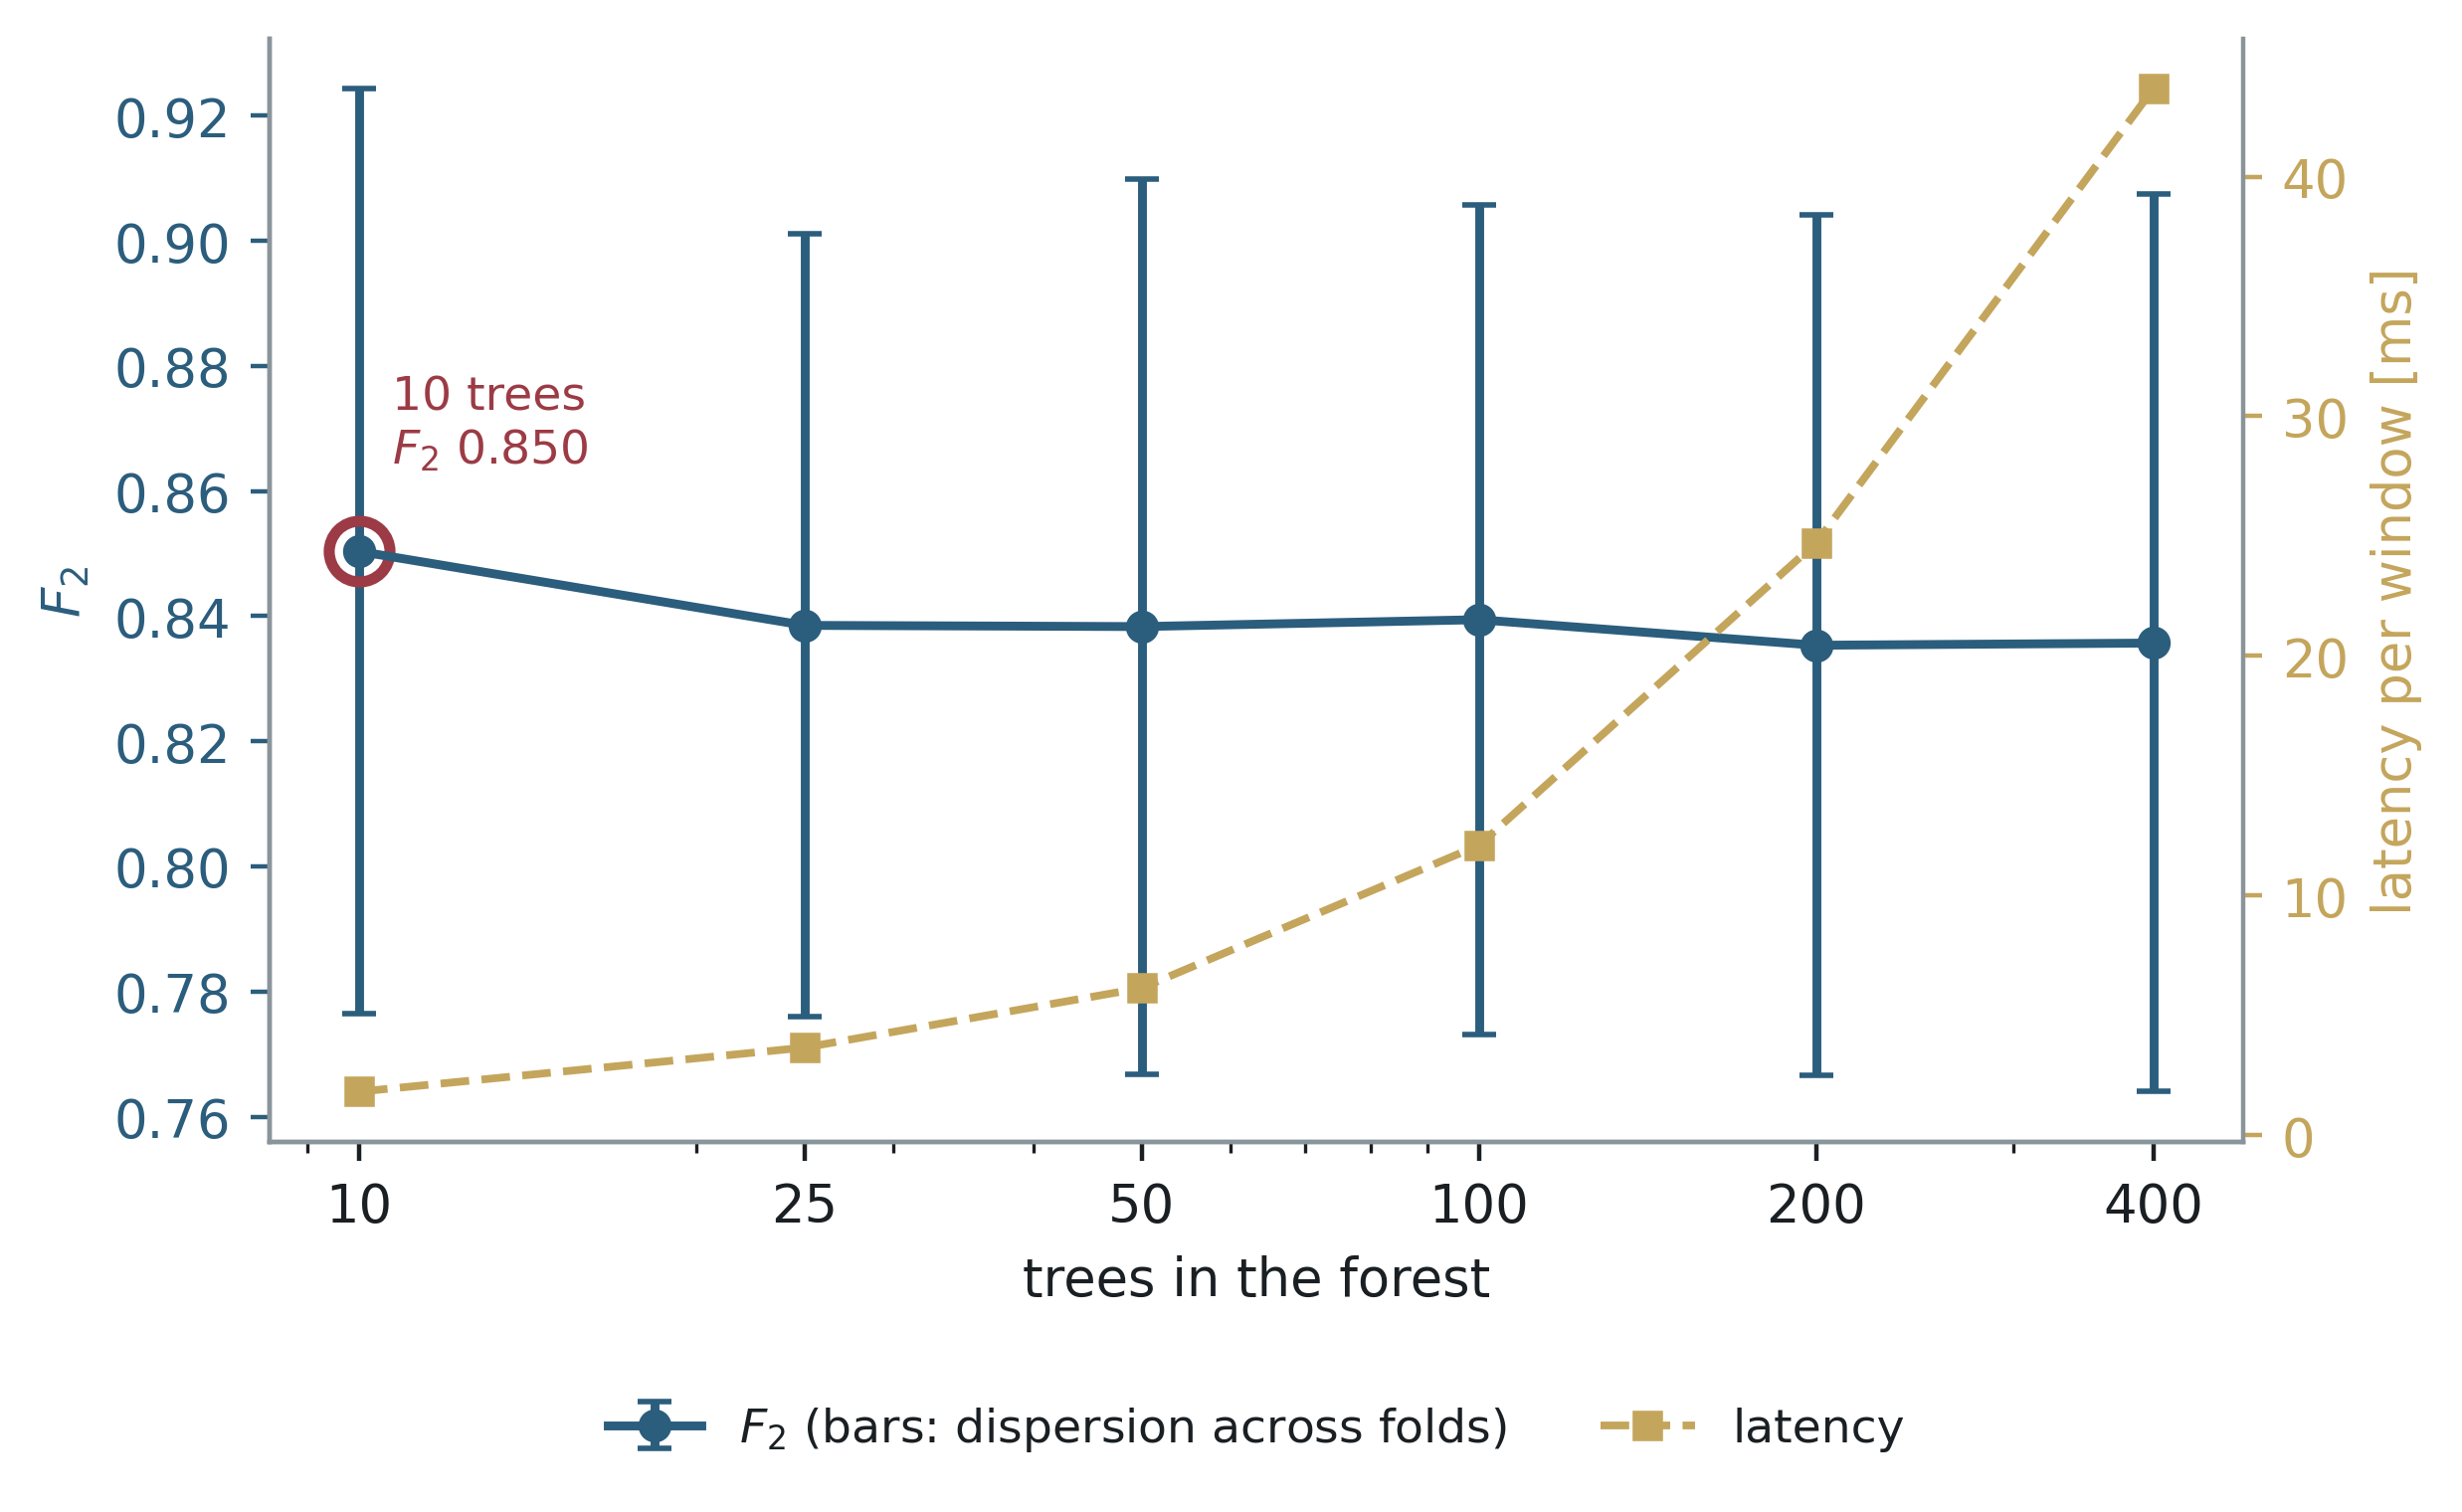
\includegraphics[width=\textwidth]{figure/fig_dimensione_en.png}
    \caption{Performance and latency as the number of trees of the
    Random Forest varies, over the 10 LOSO folds. The error bars represent the dispersion across subjects.}
    \label{fig:dimensione}
\end{figure}

With 10 trees $F_2=0{,}850\pm0{,}074$ is obtained, with 50 trees $0{,}838\pm0{,}072$ and with 400 trees $0{,}836\pm0{,}072$. The whole variation is about 0,015, against a dispersion across subjects of about 0,07. The computational cost, by contrast, changes markedly: the time per window goes from about 1,8~ms with 10 trees to 43,7~ms with 400, while the number of nodes grows from 1.881 to 76.065.

The highest mean value of $F_2$ is obtained with 10 trees, but the difference with respect to the other configurations is very small compared with the variability between subjects, and the corresponding dispersion bars overlap widely.
The trials therefore show no improvement in performance from increasing the size of the forest. We keep 50 trees, that is the configuration already in use, without regarding it as an optimal value.

\subsection{Effect of the frame rate}
\label{sec:framerate}

Another parameter analysed is the frequency at which the samples are
supplied to the classifier. UP-Fall is acquired at about 18~fps, whereas the
configuration intended for the device uses about 9 samples per second.
The effect of halving the frequency was therefore verified. This trial belongs to the preliminary five-subject configuration and is the only sensitivity analysis in the section that was not subsequently repeated on the ten subjects.

\begin{table}[ht]
\centering
\caption{Effect of halving the frame rate in the 5-subject configuration.}
\label{tab:framerate}
\begin{tabular}{lcc}
\toprule
 & \textbf{18 fps} & \textbf{9 fps} \\
\midrule
Missed falls & 6,8\% & 12,4\% \\
Variation of $F_2$ & -- & $-0{,}045$ \\
\bottomrule
\end{tabular}
\end{table}

Halving the frequency, missed falls go from 6,8\% to 12,4\%, while $F_2$ decreases by about 0,045. The loss therefore concerns recall above all. The variation of $F_2$ is smaller because the reduction in recall is partly offset by precision. Here too the overall metric alone cannot describe the behaviour of the classifier fully.

The effect of the time interval used in computing the derivatives was moreover verified. The final pipeline uses the $\Delta t$ derived from the actual timestamps instead of the nominal frequency. With respect to the computation based on a fixed 18~fps, the mean difference of $F_2$ over the ten subjects is $-0{,}006$, with $t=-1{,}15$.

The effect is therefore small. This is consistent with the features selected: of the twelve features used, eight are integral, two static and only two are derivatives and depend directly on the value of $\Delta t$. The frequency of 9~fps is kept as the reference for execution on the board, where the frequencies actually obtained are analysed in Chapter~\ref{cap:edge}.

\subsection{Length of the temporal window}
\label{sec:lunghezza_finestra}

The configuration adopted uses windows of $L=22$ samples, about 2,44~s at 9~fps. The median duration of the fall transition is, however, about 3,11~s. It was therefore verified whether a longer window might contain the whole movement better. Four lengths were compared: 22, 28, 36 and 44 samples.

\begin{figure}[htbp]
\centering 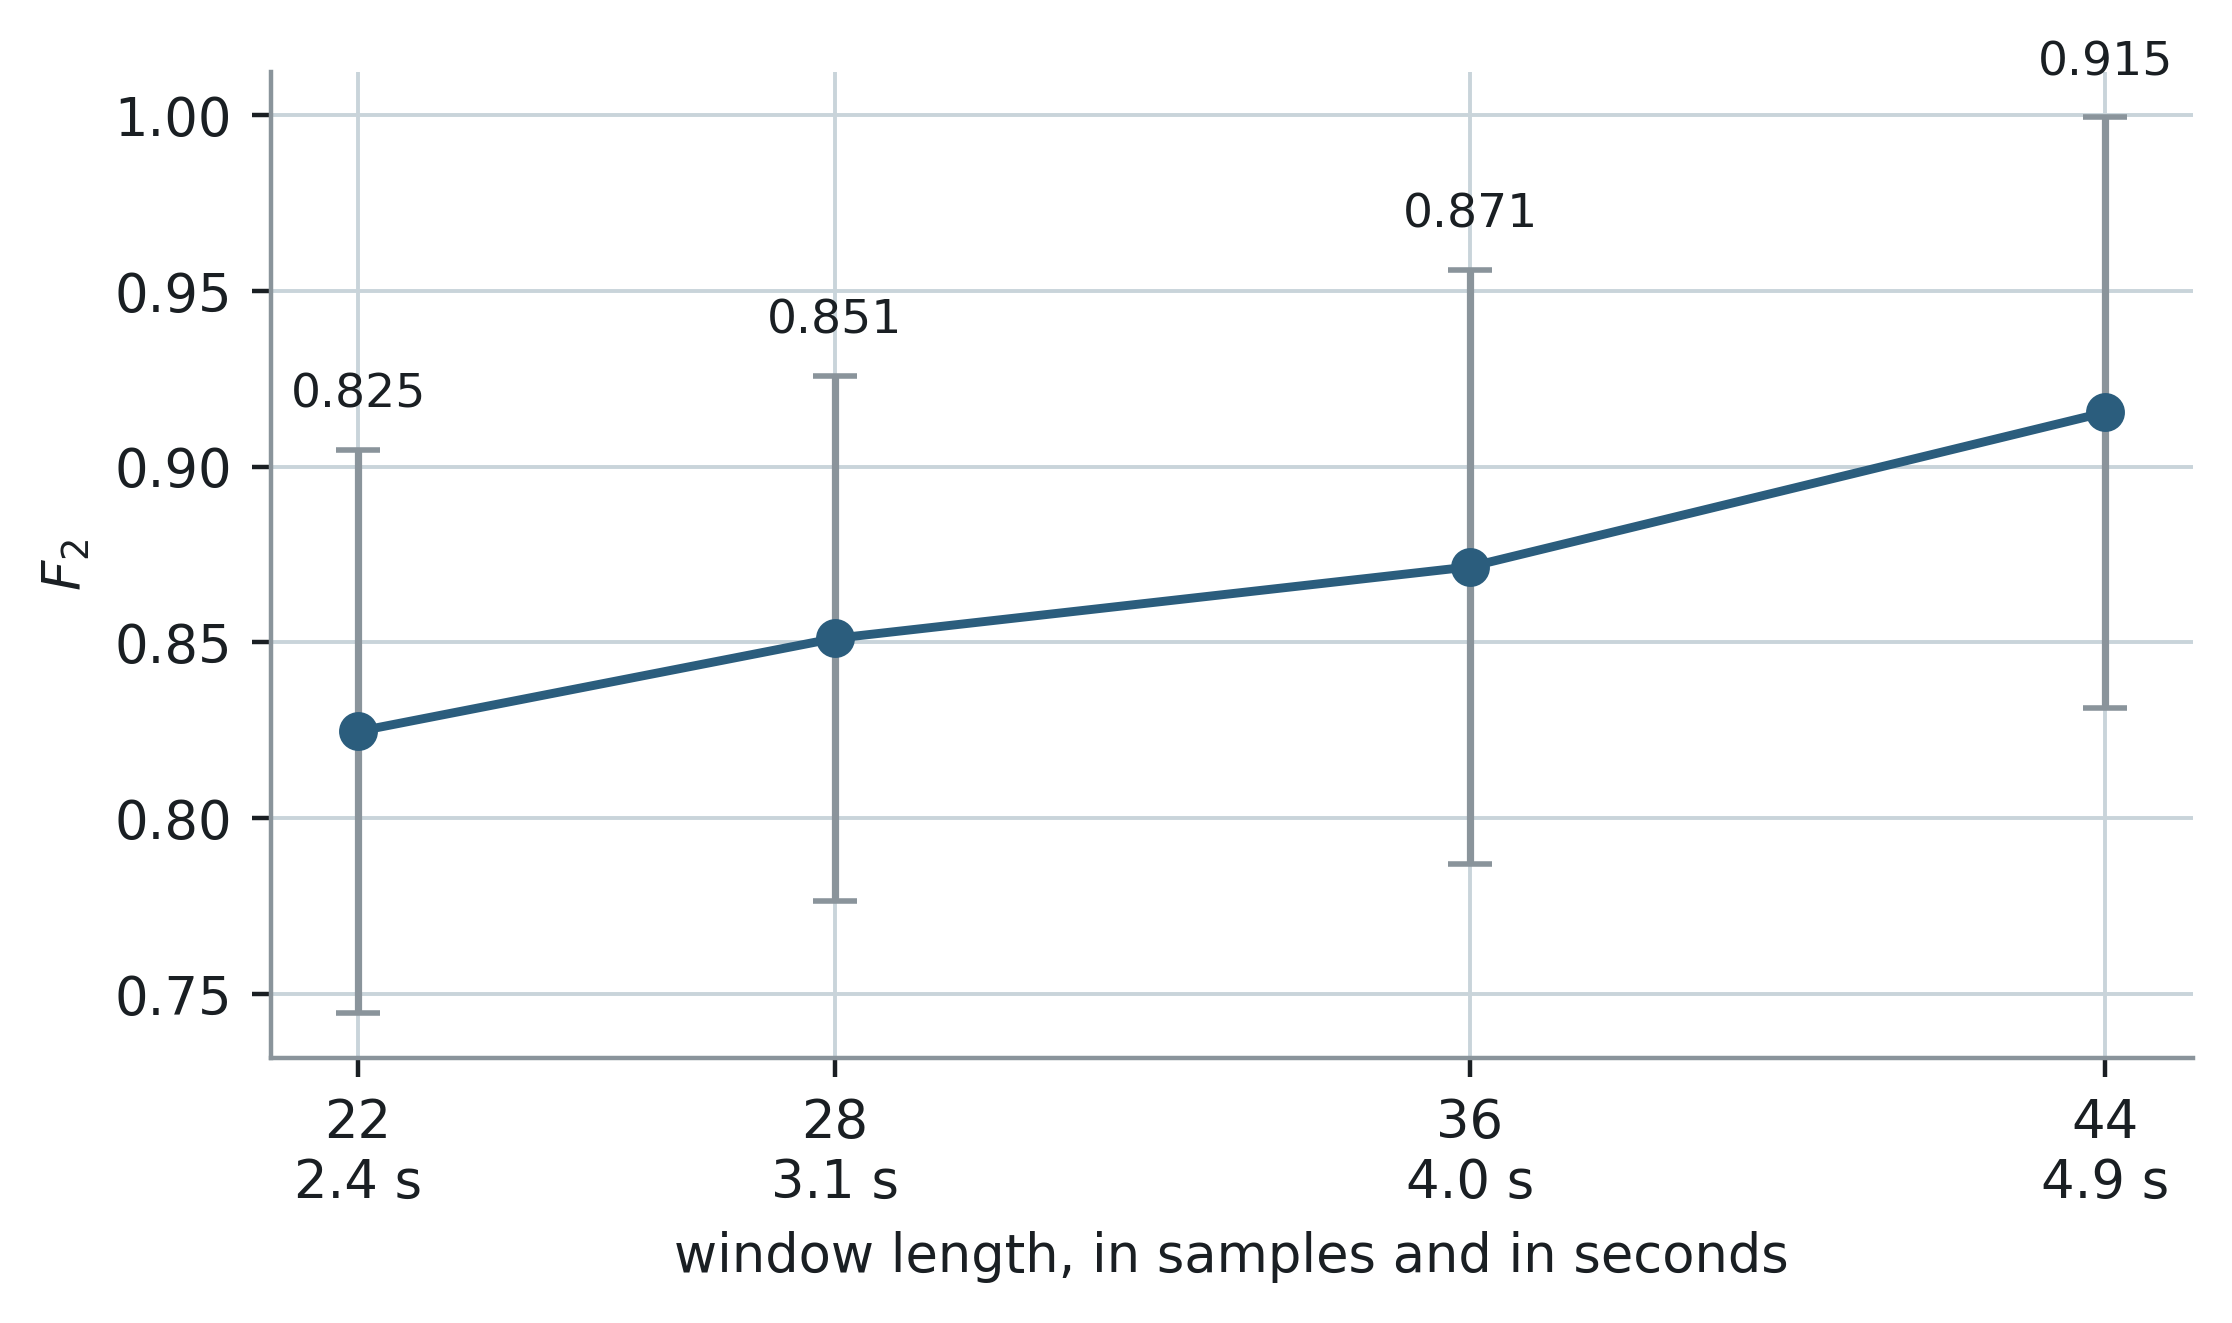
\includegraphics[width=\textwidth]{figure/fig_finestra_en.png}
\caption{Mean value of $F_2$ as the length of the window varies, over the ten LOSO folds.}
\label{fig:finestra}
\end{figure}

\begin{table}[htbp]
\centering
\caption{Performance as the length of the temporal window varies.}
\label{tab:finestra}
\begin{tabular}{ccccc}
\toprule
\textbf{$L$} & \textbf{Duration} & \textbf{$F_2$} & \textbf{Recall} & \textbf{FN / FP} \\
\midrule 22 & 2,4 s & $0{,}825 \pm 0{,}080$ & 0,849 & 232 / 468 \\
28 & 3,1 s & $0{,}851 \pm 0{,}075$ & 0,880 & 164 / 414 \\
36 & 4,0 s & $0{,}871 \pm 0{,}085$ & 0,900 & 113 / 341 \\
44 & 4,9 s & $0{,}915 \pm 0{,}084$ & 0,945 & \phantom{0}53 / 249 \\
\bottomrule
\end{tabular}
\end{table}

Performance increases steadily with the length. Going from 22 to 44 samples, $F_2$ rises from 0,825 to 0,915 and recall from 0,849 to 0,945.
False negatives and false positives decrease at the same time, from 232 to 53 and from 468 to 249 respectively. The improvement is therefore not due solely to a shift in the trade-off between precision and recall.

The paired comparison between 22 and 44 samples produces a mean difference of $+0{,}091$ of $F_2$, with $t=3{,}62$.
Despite this result, $L=22$ is retained in the final configuration. A window of 44 samples requires about 4,9~s before a decision can be produced, against 2,44~s with 22 samples.
The choice is therefore a compromise between performance on the benchmark and the time needed to collect the sequence. The contribution of the window to the overall latency is measured in Chapter~\ref{cap:edge}.

\subsection{Sensitivity to the loss of landmarks}
\label{sec:occlusioni}

The availability of the landmarks may be reduced when some parts of the body are not detected by the pose estimator. In order to verify how far this can affect classification, a controlled simulation was carried out in which certain points of the body were made unavailable.

 The landmark treated as unavailable is held at the last value observed instead of being set to zero, thereby avoiding an artificial displacement towards the origin of the image. Both anatomical groups and random groups of increasing size were tried. The configuration without occlusions has $F_2=0{,}853\pm0{,}071$.

\begin{table}[htbp]
\centering
\caption{Variation of $F_2$ obtained by freezing different groups of landmarks.}
\label{tab:occlusioni}
\begin{tabular}{lcc}
\toprule
\textbf{Group} & \textbf{Points} & \textbf{$\Delta F_2$} \\
\midrule
Shoulders & 2 & $-0{,}037$ \\
Ankles & 2 & $-0{,}012$ \\
Left half & 6 & $-0{,}004$ \\
Nose & 1 & $-0{,}002$ \\
Knees + ankles & 4 & $+0{,}001$ \\
Hips & 2 & $+0{,}015$ \\
\midrule
Random 11\% & 1 & $-0{,}002$ \\
Random 22\% & 2 & $+0{,}001$ \\
Random 33\% & 3 & $+0{,}003$ \\
Random 55\% & 5 & $-0{,}032$ \\
\bottomrule
\end{tabular}
\end{table}

\begin{figure}[htbp]
\centering
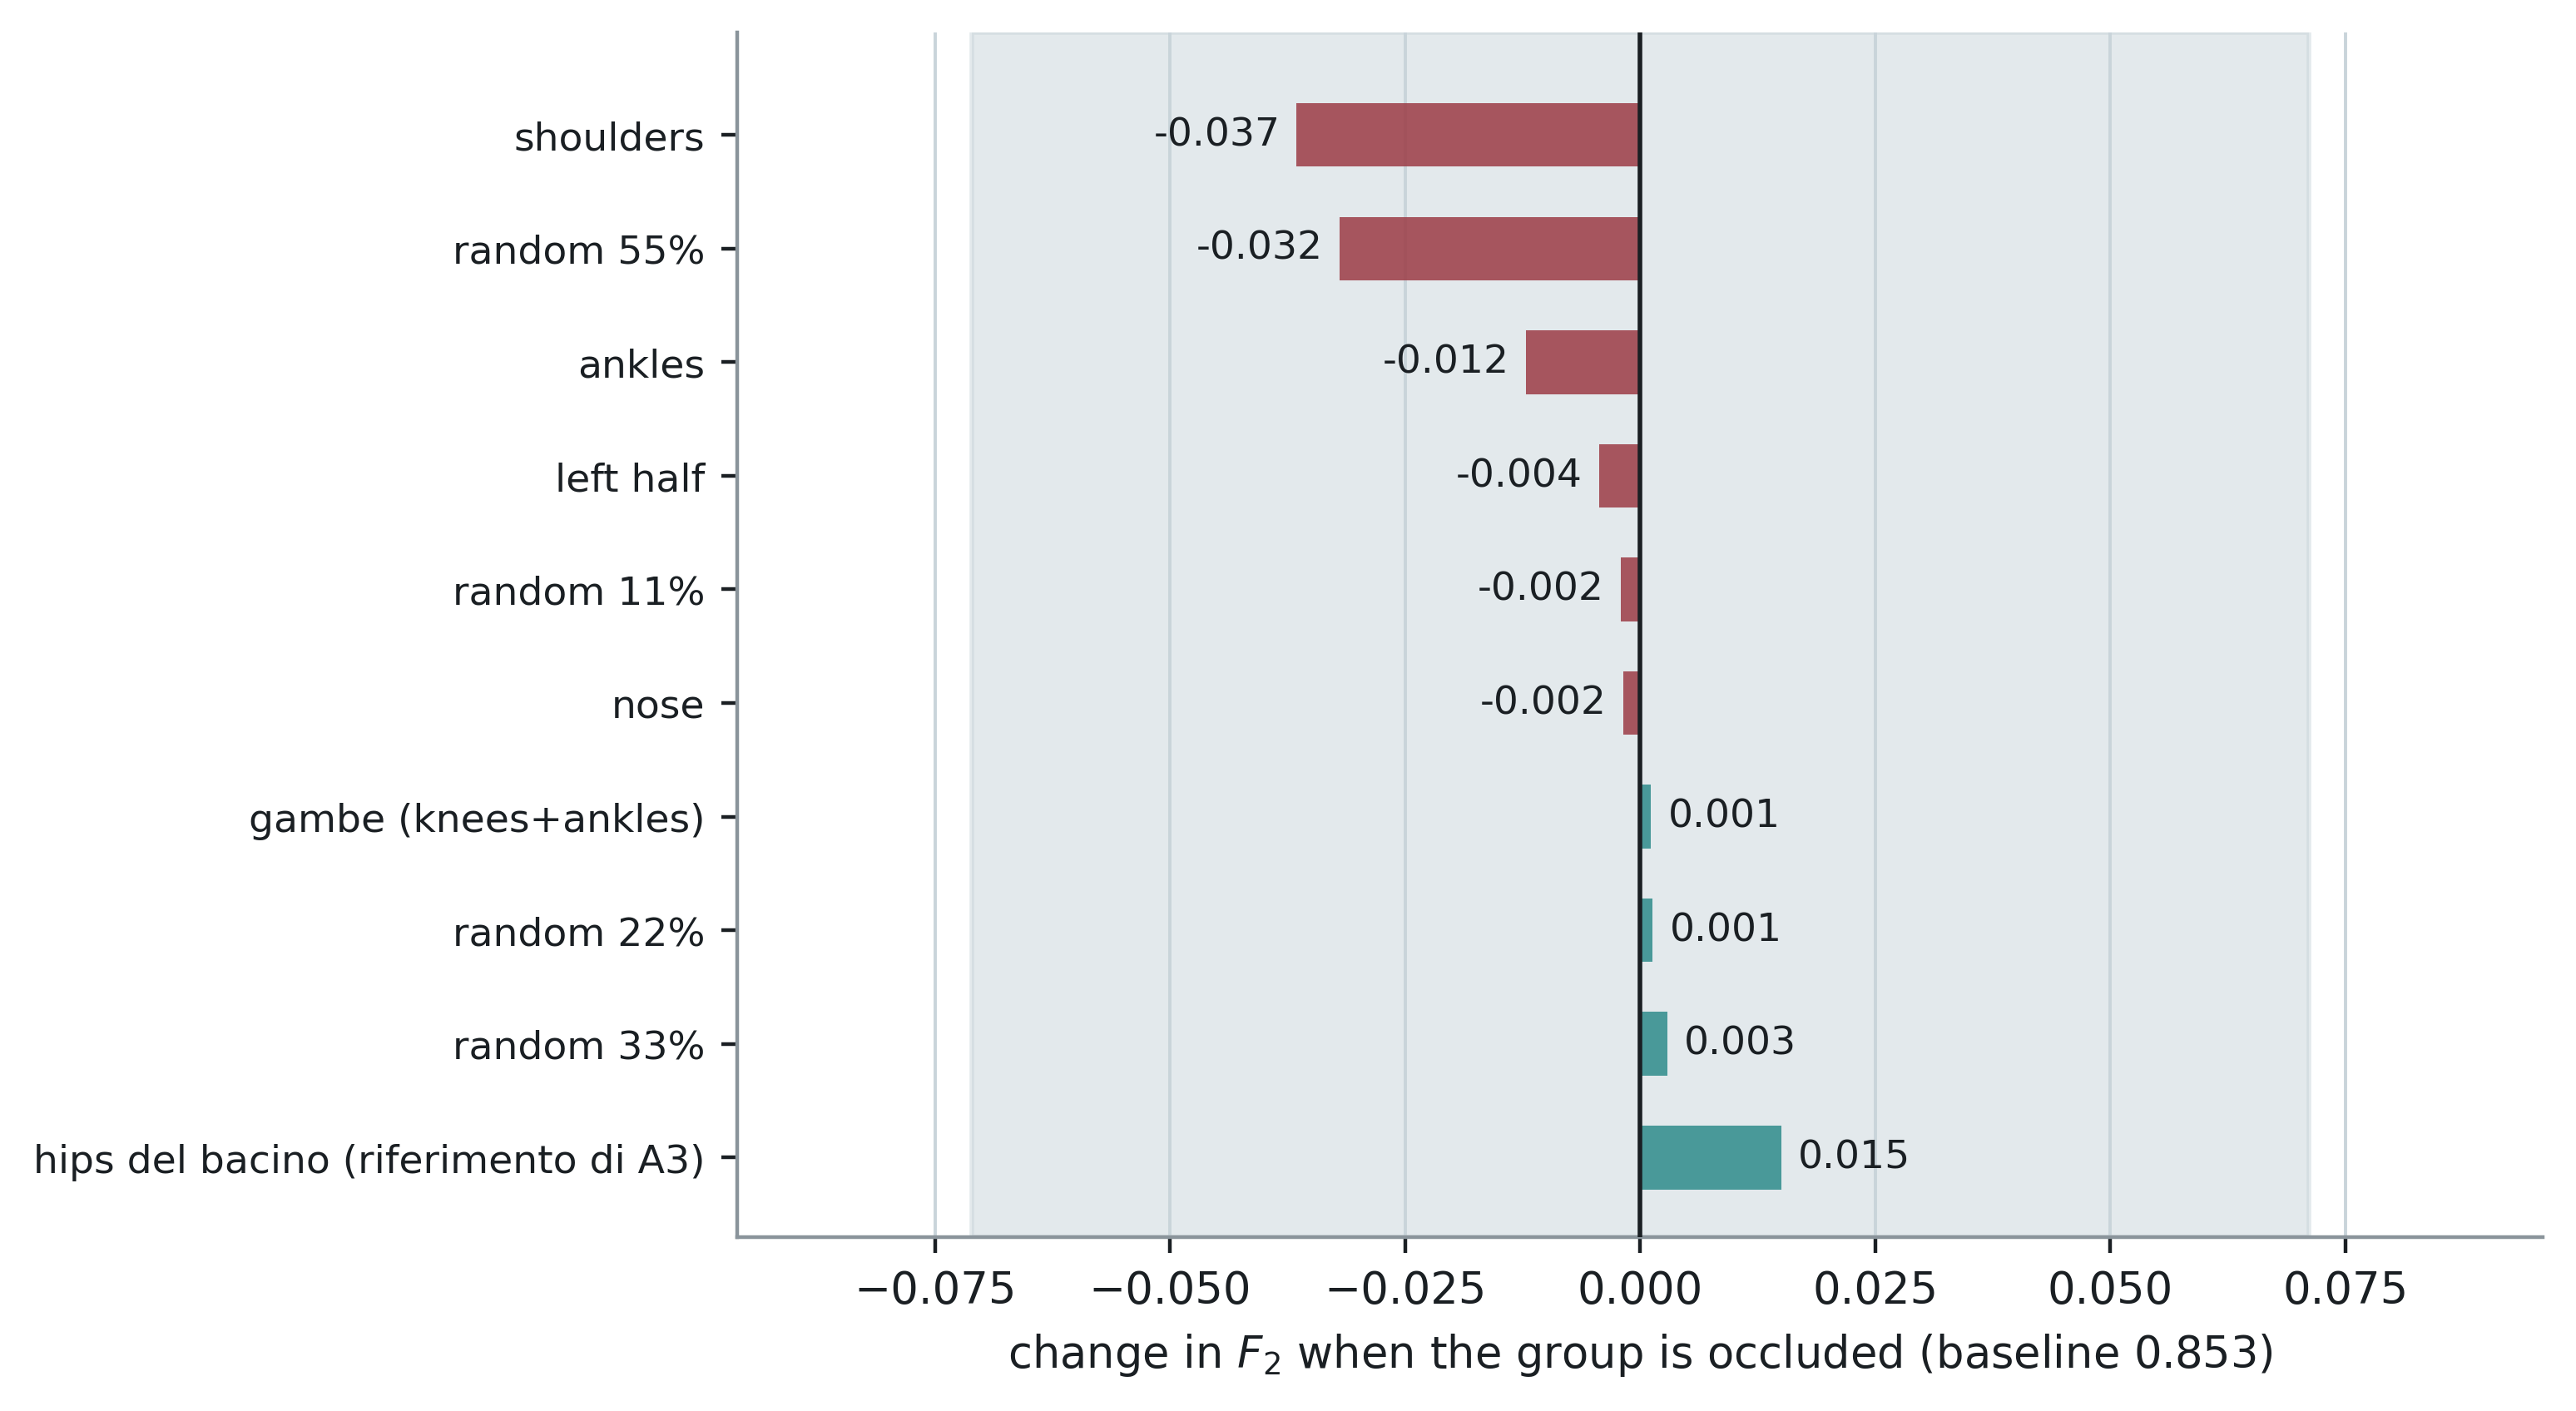
\includegraphics[width=0.86\textwidth]{figure/fig_occlusioni_en.png}
\caption{Effect of the simulated occlusions on the different groups of landmarks.}
\label{fig:occlusioni}
\end{figure}

The largest degradation is 0,037 of $F_2$ and is obtained by masking the shoulders. This value is about half the dispersion across subjects, 0,071. None of the groups considered therefore causes, on its own, a variation larger than the variability already present between people.
The small positive variations are not interpreted as improvements, but as experimental fluctuations.

Among the anatomical groups, the largest variation is observed by masking the shoulders.
Repeating the same trial with the previous subset of features, however, the loss goes from $-0{,}037$ to $-0{,}019$. Sensitivity therefore also depends on the features built from the landmarks.
A particular case concerns the hips. When their position is not updated, some features of representation A3 remain indirectly referred to a more stable position in the image plane. With a fixed camera this may reintroduce part of the information about the position of the person in the scene.

The experiment had not, however, been designed to assess the feature $h_{\text{pav}}$ directly, and cannot therefore be regarded as a verification of its effectiveness. The trial concerns simulated occlusions in any case, and does not warrant the conclusion that the system is robust to extensive real occlusions.

\subsection{Temporal regularity of the quantities}
\label{sec:autocorrelazione}

In order to compare the temporal regularity of the dynamic quantities, the one-step autocorrelation was measured:

\[
\rho_1 =
\frac{\operatorname{Cov}(x_t,x_{t-1})}
{\sigma_{x_t}\sigma_{x_{t-1}}}.
\]

The computation was carried out only within continuous stretches with a valid pose. The results are reported in Table~\ref{tab:autocorrelazione}.

\begin{table}[htbp]
\centering
\caption{One-step autocorrelation of the main dynamic quantities}
\label{tab:autocorrelazione}
\begin{tabular}{lc}
\toprule
\textbf{Quantity} & $\boldsymbol{\rho_1}$ \\
\midrule
\multicolumn{2}{l}{\emph{Instantaneous derivatives}} \\
\quad Variation of the trunk angle & 0,221 \\
\quad Angular velocity of the trunk & 0,494 \\
\quad Velocity of the hips & 0,499 \\
\quad Velocity of the head & 0,535 \\
\midrule
\multicolumn{2}{l}{\emph{Integral quantities}} \\
\quad Descent of the hips & 0,818 \\
\quad Path of the hips & 0,882 \\
\quad Excursion of the trunk & 0,988 \\
\bottomrule
\end{tabular}
\end{table}

The derivatives have values between 0,221 and 0,535, while the integral quantities range between 0,818 and 0,988. Even the lowest value of the integral quantities remains above the highest value of the derivatives, and they are therefore more regular over time. This comparison describes, however, only the continuity of the signals, and does not show that a feature with a higher autocorrelation is also more useful for classification.

\subsection{Sensitivity to landmark noise}
\label{sec:rumore}

Finally, the sensitivity to noise in the coordinates of the landmarks was verified.
Errors in pose estimation were simulated by adding independent Gaussian noise. The standard deviation $\sigma$ is expressed as a fraction of the length of the torso, so as not to depend on the apparent size of the person in the image.

Three configurations were compared: the representation without the integral quantities (A3base), the complete one (A3) and the subset selected by DTW (DTW). The results are reported in Table~\ref{tab:rumore} and in Figure~\ref{fig:rumore}.

\begin{table}[htbp]
\centering
\caption{Value of \(F2\) as the Gaussian noise added to the landmarks increases.}
\label{tab:rumore}
\begin{tabular}{lccc}
\hline
$\boldsymbol{\sigma}$ & \textbf{without integrals (10)} & \textbf{with integrals (13)} & \textbf{selected subset (12)}\\
\hline
0     & 0,874 & 0,858 & 0,857 \\
0,005 & 0,863 \,(--0,011) & 0,864 \,(+0,006) & 0,844 \,(--0,012) \\
0,010 & 0,855 \,(--0,018) & 0,866 \,(+0,008) & 0,863 \,(+0,007) \\
0,020 & 0,864 \,(--0,010) & 0,846 \,(--0,012) & 0,836 \,(--0,021) \\
0,040 & 0,863 \,(--0,011) & 0,856 \,(--0,002) & 0,825 \,(--0,031) \\
\hline
\end{tabular}
\end{table}

\begin{figure}[htbp]
\centering
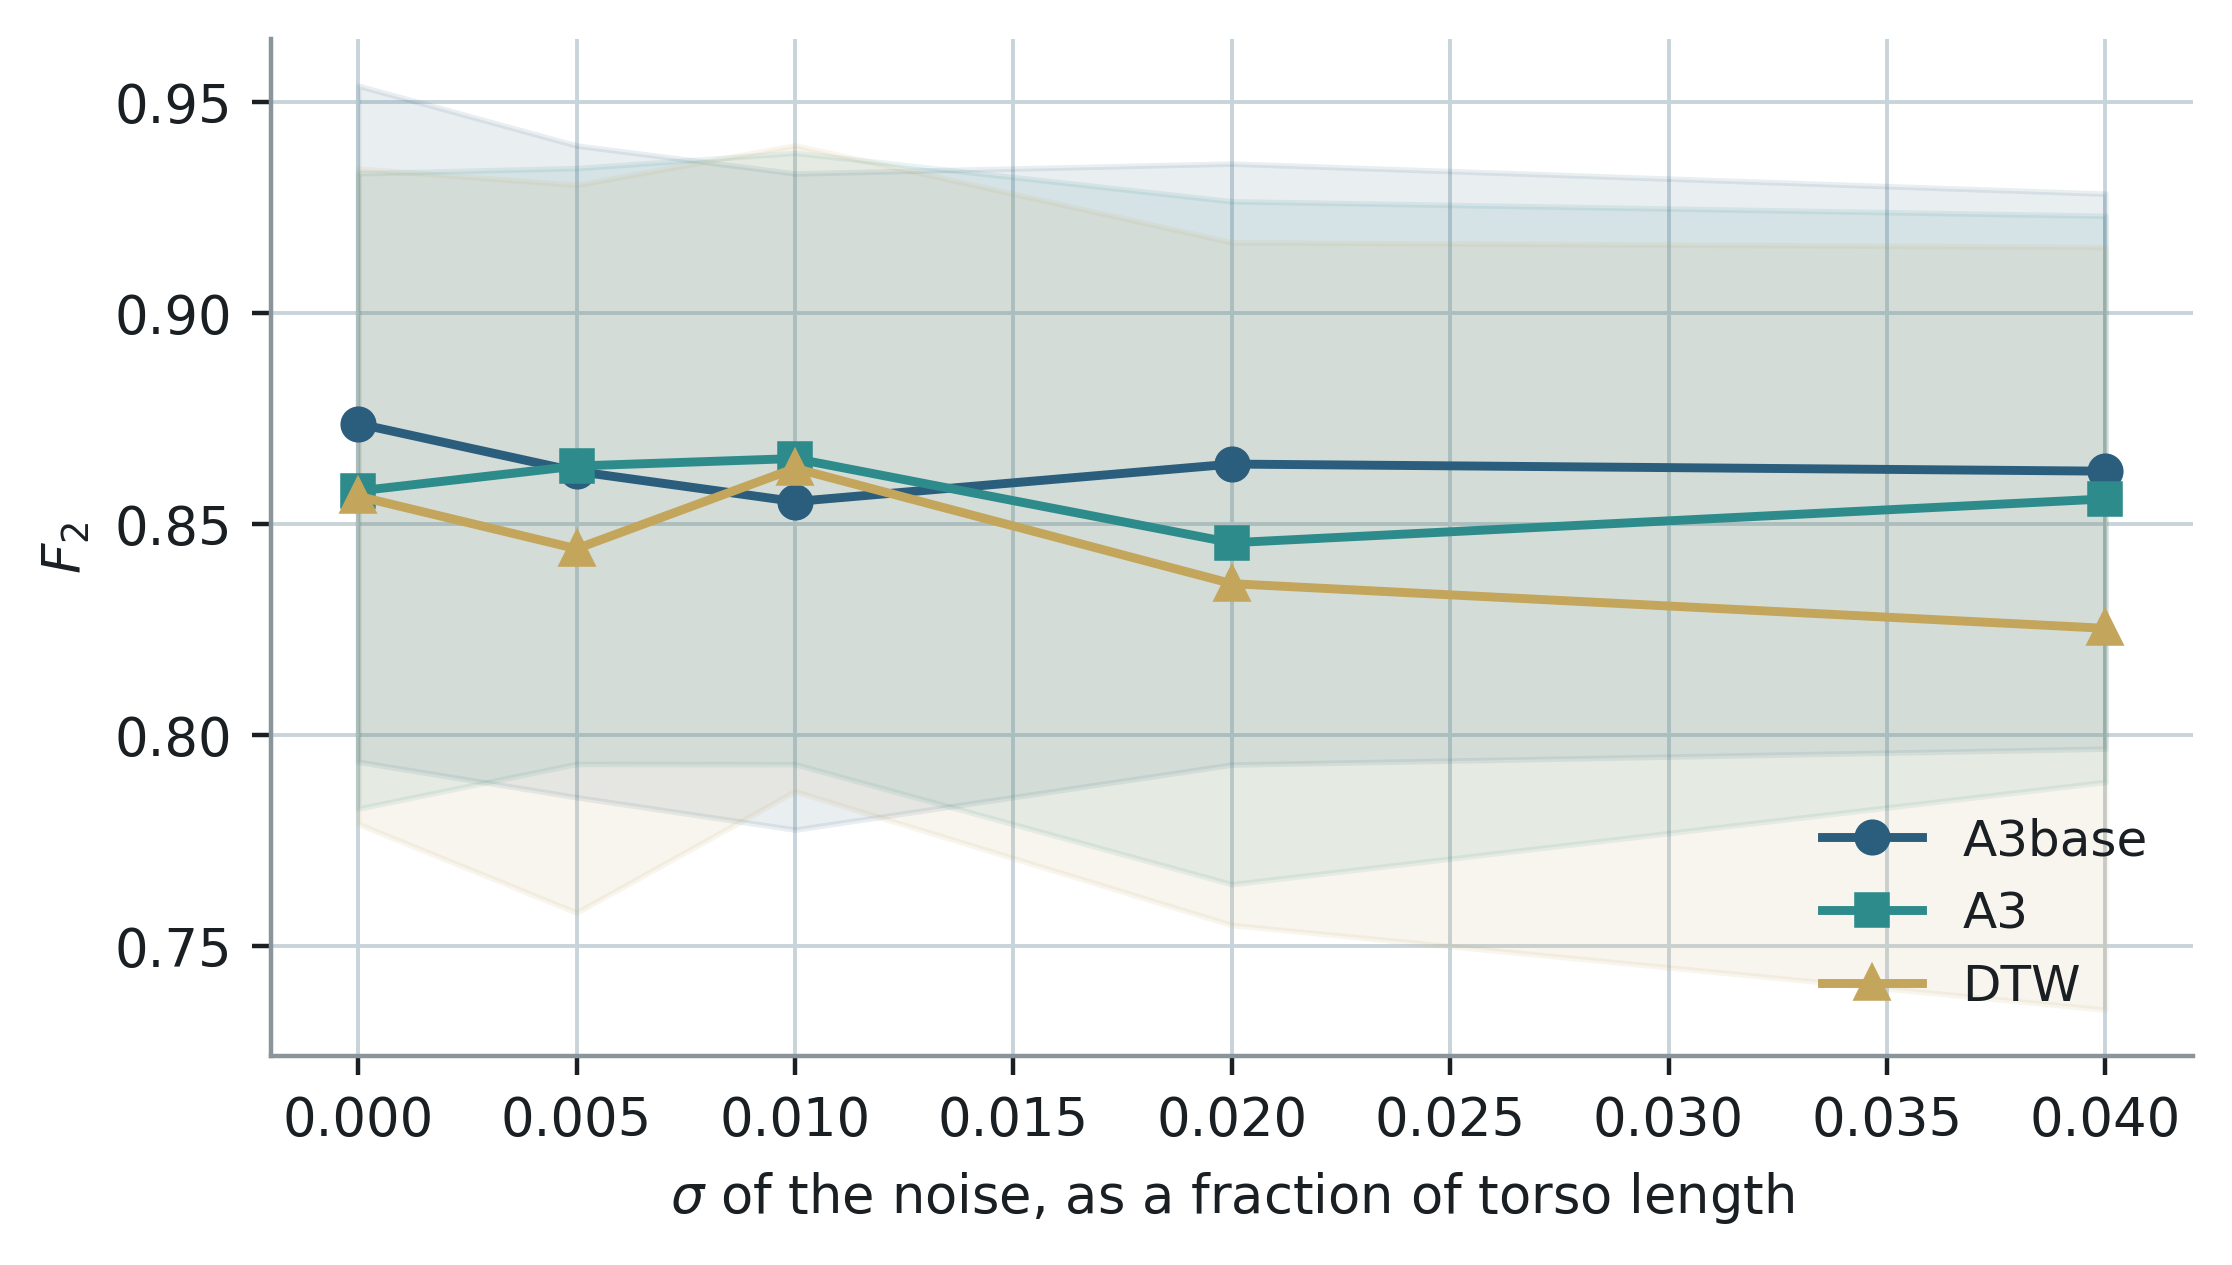
\includegraphics[width=0.86\textwidth]{figure/fig_rumore_en.png}
\caption{Performance as the Gaussian noise added to the coordinates of the landmarks increases, for the three feature sets considered.}
\label{fig:rumore}
\end{figure}

Even with \(\sigma=0{,}04\), the largest degradation is 0,031 of $F_2$, therefore below the dispersion across subjects, which is about 0,08.
Nor do the integral quantities show a greater degradation than the instantaneous quantities alone: between the representation without integral quantities and the complete one, that is at parity of everything except the three integral quantities, the degradation at $\sigma=0{,}04$ is $0{,}011$ and $0{,}002$ respectively. The positive variations observed at intermediate noise levels are fluctuations within the dispersion between subjects, and are not interpreted as improvements.

This result does not mean that the integral quantities eliminate the noise. Path, excursion and descent still depend on the coordinates of the landmarks and may therefore vary when these are perturbed. Under the conditions considered, however, independent Gaussian noise has a limited effect on the final performance. In the domestic recordings a different error was instead observed. In some cases the estimator switches from one plausible configuration of the pose to another, and the new configuration remains coherent for several frames. This behaviour can be interpreted by the temporal features as real movement. One example was observed on the excursion of the trunk, as reported in Table~\ref{tab:ambiguita}.

\begin{table}[htbp]
\centering
\caption{Excursion of the trunk over a sliding window in two domestic recordings.}
\label{tab:ambiguita}
\begin{tabular}{lcc}
\hline
 & \textbf{Median} & \textbf{Maximum} \\
\hline
Person still on a sofa & 9,0$^\circ$ & 93,5$^\circ$ \\
Fall & 9,0$^\circ$ & 60,7$^\circ$ \\
\hline
\end{tabular}
\end{table}

In this case a person who is still produces a maximum excursion greater than that of the fall. The increase does not correspond to real movement of the body, but to the estimator switching between two different poses. Gaussian noise therefore does not reproduce all the errors that may appear during real operation. If a wrong pose remains stable for several frames it can be interpreted as real movement by the integral quantities too, and even a temporal filter may not be enough to correct it.

\section{Effect of the definition of the task}
\label{sec:compito-risultati}

So far the definition of the positive class has been kept unchanged. In this analysis the task assigned to the classifier is instead modified, distinguishing the fall transition from the subsequent state in which the person remains on the ground. Three tasks were considered:
\begin{enumerate}
\item \emph{event}: only the fall transition is positive;
\item \emph{state}: only the post-fall state is positive;
\item \emph{alarm}: transition and post-fall state are both considered positive.
\end{enumerate}

Model, features and protocol are kept unchanged. What changes is the prevalence of the positive class in the training set, because the three formulations use different portions of the fall episode. In order to make the results comparable, all the models are evaluated on the same alarm label, which treats both the transition and the post-fall state as positive.

Greater attention was paid in the analysis to the windows in which the person lies down voluntarily, because they are hard cases to distinguish from the post-fall state, the final configuration of the body being very similar to that of a person who has remained on the ground after a fall. Precisely in order to isolate them, the three tasks are defined on the OmniFall annotations introduced in
Section~\ref{sec:compito}, and not on the hand-made labels: the latter assign the normal class to every frame of the daily-activity recordings, and therefore cannot separate voluntary lying down from the rest. The classes \texttt{fall} and \texttt{fallen} do make it possible, and a window turns out positive when it contains at least five of their frames.

The resulting set does not coincide with the one used in the comparisons between
architectures and representations: it comprises 12.140 windows, of which
1.399 are positive, that is $11{,}5\%$, against the 11.719 windows and
1.491 positives ($12{,}72\%$) of Section~\ref{sec:metriche}. The same
definition of the positive is adopted in the sensitivity analyses of
Sections~\ref{sec:occlusioni} and~\ref{sec:rumore}, and is the reason why the
reference values reported there do not coincide with those of
Table~\ref{tab:architetture}.

\begin{table}[htbp]
\centering
\caption{Performance obtained with the three definitions of the task, keeping model, features and protocol unchanged.}
\label{tab:compiti}
\small
\begin{tabularx}{\textwidth}{@{}l c c c c >{\centering\arraybackslash}X@{}}
\toprule
\textbf{Task} &
\textbf{Train. prev.} &
\textbf{$F_2$} &
\textbf{Recall} &
\textbf{Precision} &
\textbf{Hard negatives} \\
\midrule
Event  & 0,047 & $0{,}415 \pm 0{,}083$ & 0,364 & 0,990 & \phantom{0}0,04\% \\
State   & 0,089 & $0{,}587 \pm 0{,}094$ & 0,552 & 0,874 & \phantom{0}8,4\% \\
Alarm & 0,115 & $0{,}830 \pm 0{,}066$ & 0,836 & 0,841 & 11,7\% \\
\bottomrule
\end{tabularx}
\end{table}

\begin{figure}[ht]
\centering
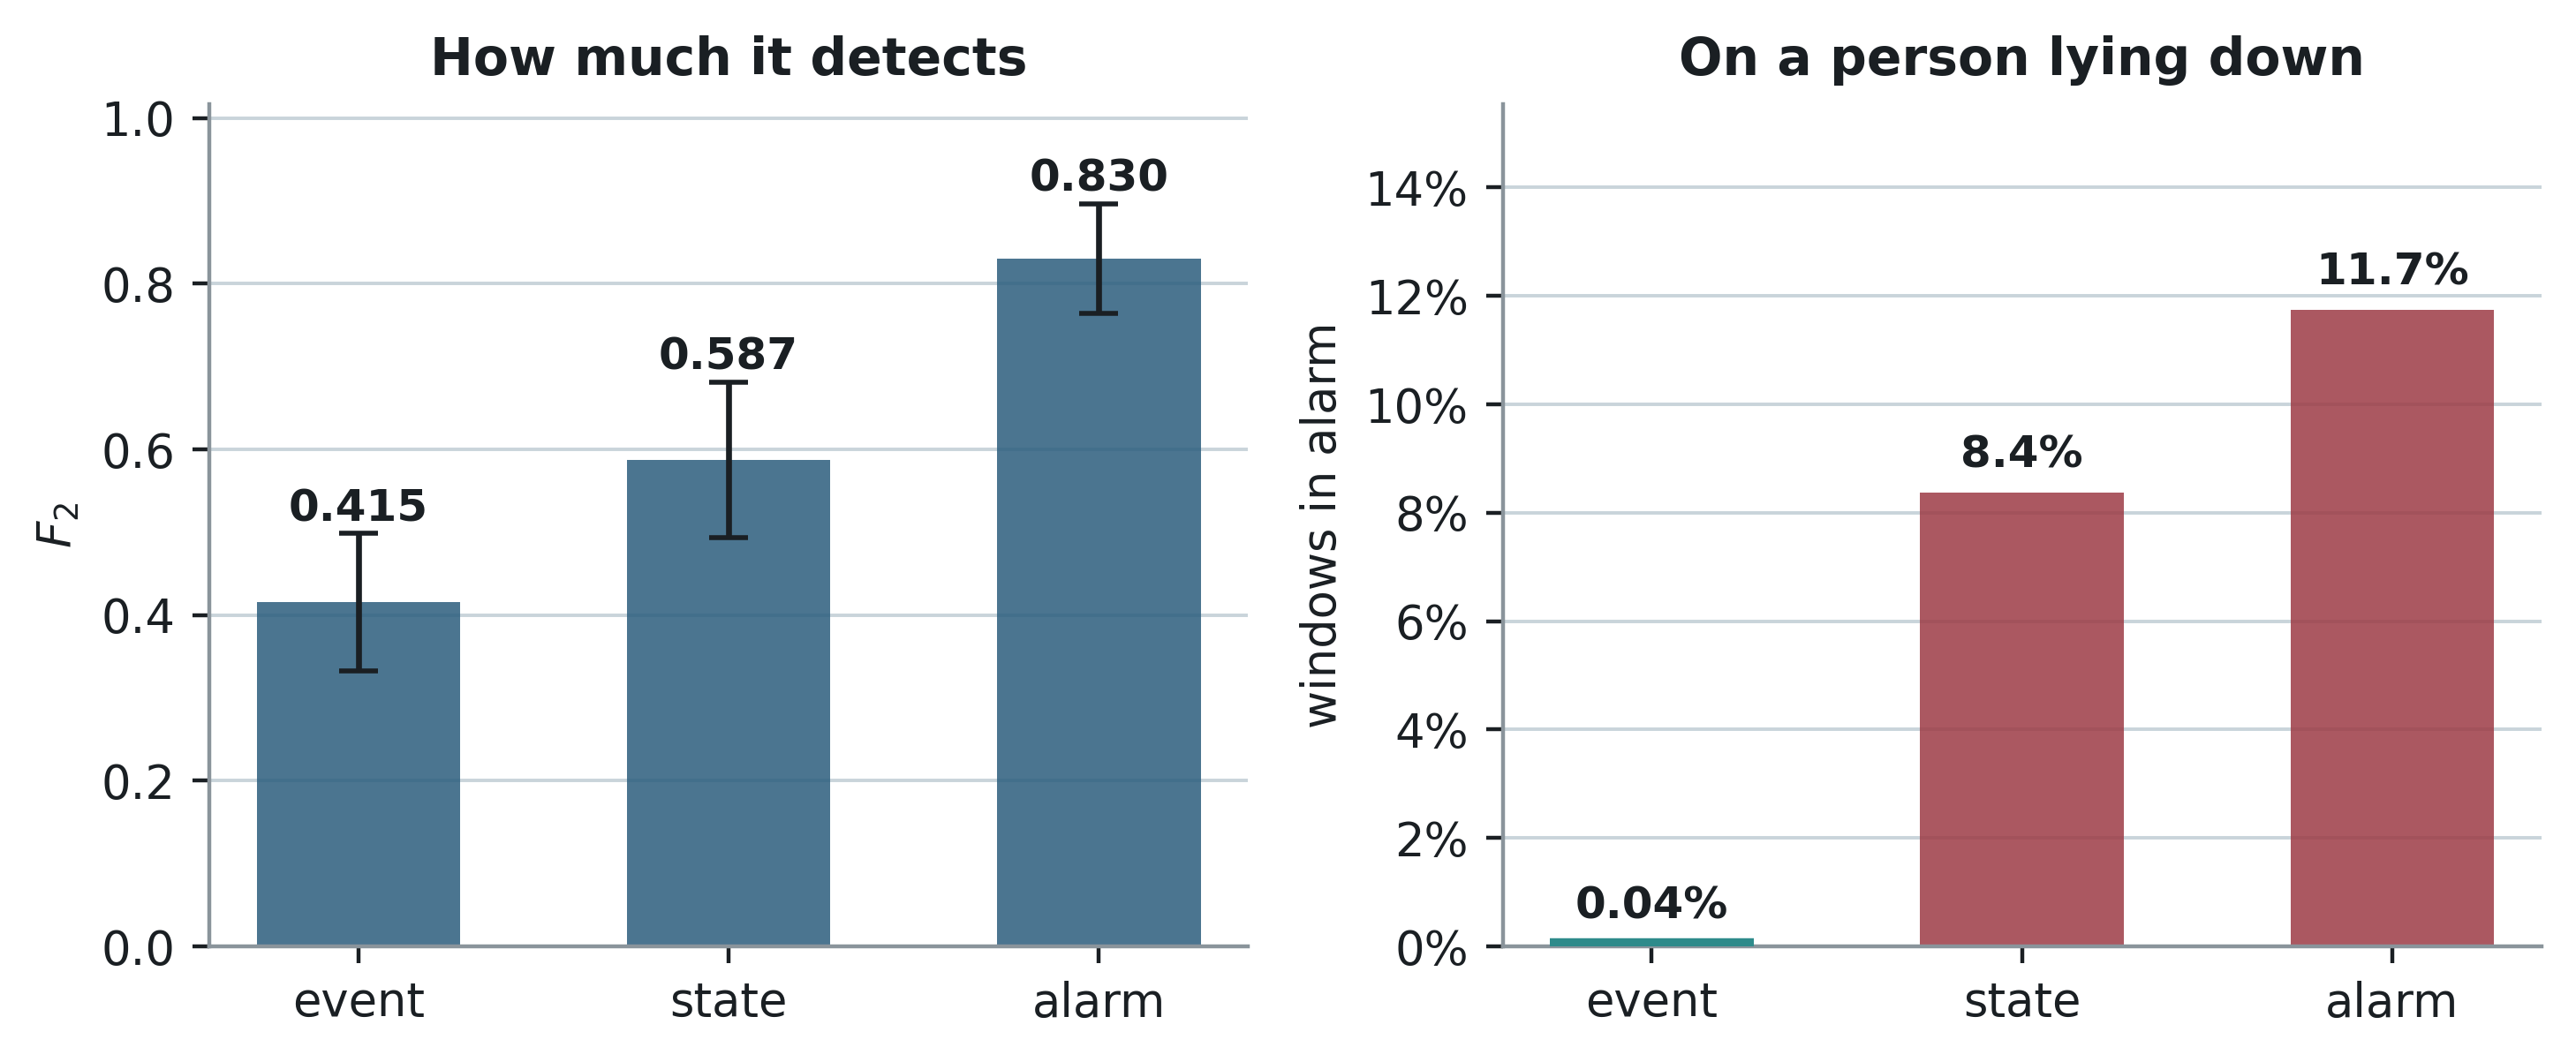
\includegraphics[width=\textwidth]{figure/fig_compiti_en.png}
\caption{Comparison between the three definitions of the task. On the left
$F_2$ is reported; on the right the share of windows flagged as positive
during the act of lying down voluntarily.}
\label{fig:compiti}
\end{figure}

The \emph{alarm} formulation reaches the highest mean value of $F_2$, 0,830, and the highest recall, 0,836. The \emph{state} task reaches 0,587, while the \emph{event} task stops at 0,415.

The difference concerns recall above all. The model trained on the transition alone recognises less often the windows in which the person is already on the ground, which are nonetheless treated as positive in the common evaluation. Precision instead shows the opposite behaviour. The event task reaches 0,990 and classifies as positive only one of the 2.234 windows relating to lying down voluntarily. The share rises to 8,4\% for the state task and to 11,7\% for the alarm task.

The three formulations therefore produce a different trade-off between recall and false positives. The \emph{event} task is more selective, but loses part of the positive windows. The \emph{alarm} task increases recall and $F_2$, but introduces more errors in the activities that end in a posture similar to the post-fall state. The definition of the task therefore has a considerable effect on the results, greater than the one observed by changing the architecture of the classifier alone. The operational behaviour of the three formulations is taken up again in Chapter~\ref{cap:edge}, where the comparison is made at the level of events and of false alarms per hour.

\subsection{Dynamics of the fall and voluntary lying down}

A fall and the voluntary act of lying down may bring the person into a similar final position, but they differ in the movement that precedes it.
In the definition of the task it is possible to treat as the positive class the \emph{event}, that is the phase in which the fall occurs, the subsequent \emph{state}, when the person is already on the ground, or both conditions for the purposes of the alarm.

This distinction matters because the final configuration of the body may be similar in the two cases, whereas the dynamics by which it is reached may be very different. In order to verify this difference, some dynamic quantities were compared during the transition and during the subsequent state on the ground. The ratios between the medians are reported in Table~\ref{tab:dinamica}.

\begin{table}[htbp]
\centering
\caption{Ratio between the medians of the dynamic quantities in the phases considered.}
\label{tab:dinamica}
\begin{tabular}{lcc}
\toprule
\textbf{Quantity} &
\textbf{Fall / lying down} &
\textbf{On the ground / lying} \\
\midrule Velocity of the hips & 30,1$\times$ & 1,3$\times$ \\
Excursion of the trunk & 42,5$\times$ & 2,8$\times$ \\
Path of the hips & 33,0$\times$ & 1,3$\times$ \\
Descent of the hips & 139,4$\times$ & 2,1$\times$ \\
\bottomrule
\end{tabular}
\end{table}

During the transition the differences are very marked. The velocity of the hips is about 30 times greater during a fall, while for the descent of the hips the ratio reaches 139,4. Comparing the two final states, by contrast, the ratios fall to values between 1,3 and 2,8. What is most discriminative is therefore not the final position alone, but the movement by which the person reaches that position.

\section{Verification of the methodological choices}
\label{sec:misura_leakage}

Chapter~\ref{cap:metodologia} pointed out two choices that also used information coming from subjects subsequently employed in the test: the choice of the parameter $K$ and feature selection. In order to assess the effect of this, both procedures were repeated within the individual folds, excluding the test subject every time.

\subsection{Choice of the parameter $K$}

For every fold, $K$ is chosen using only the nine remaining subjects, and the value selected was then evaluated on the subject left out.

\begin{table}[htbp]
\centering
\caption{Value of $K$ chosen within each fold, compared with $K=31$.}
\label{tab:k_misura}
\begin{tabular}{@{}lccc@{}}
\toprule
\textbf{Subject left out} & \textbf{$K$ chosen} & \textbf{$F_2$ with the $K$ chosen} & \textbf{$F_2$ with $K=31$} \\
\midrule 1 & 45 & 0,864 & 0,863
\\ 2 & 45 & 0,739 & 0,751
\\ 3 & 31 & 0,676 & 0,676
\\ 4 & 45 & 0,897 & 0,873
\\ 5 & 45 & 0,897 & 0,874
\\ 6 & 45 & 0,961 & 0,952
\\ 7 & 45 & 0,845 & 0,819
\\ 8 & 45 & 0,927 & 0,882
\\ 9 & 45 & 0,894 & 0,773
\\ 10 & 45 & 0,808 & 0,785
\\
\midrule
\emph{Mean} & --- & \textbf{0,851} & 0,825 \\
\bottomrule
\end{tabular}
\end{table}

Nine folds out of ten select $K=45$. Using the value chosen without the test subject, the mean $F_2$ goes from 0,825 to 0,851, a difference of 0,026. The choice of $K=31$ therefore did not produce an overestimate of the laboratory performance. In this comparison it produces, if anything, a lower mean value. The paired test returns $t=2{,}22$, just below the critical value of 2,26, and does not therefore allow the difference to be regarded as significant at the level used.

The result is influenced above all by subject 9, for whom the difference reaches 0,122. Without this subject, the mean difference drops from 0,026 to 0,016. The value of the test rises to $t=2{,}72$, but this second measurement serves only to show the weight of the individual case and does not replace the test on the ten subjects.
That $K=45$ is chosen almost every time is consistent with the scan carried out earlier: considering the laboratory trials alone, $K=45$ had produced better results than $K=31$.

$K=31$ was also retained on the basis of the first domestic trials, in which four falls out of five were recognised against three with $K=45$.
This part of the choice cannot be verified independently on the same data and is therefore retained as a limitation.

\subsection{Feature selection}
Feature selection was repeated separately for each fold, excluding the subject used for the test every time. The subset obtained was then compared with the twelve features used in the main experiments.

\begin{table}[htbp]
\centering
\caption{Feature selection repeated within each fold}
\label{tab:leakage_misura}
\small
\begin{tabularx}{\textwidth}{@{}l c X@{}}
\toprule
\textbf{Subject left out} & \textbf{In common} & \textbf{Main changes} \\
\midrule
1 & 10/12 & \texttt{A2\_percorso}, \texttt{A3\_escursione} drop out \\
2 & 11/12 & \texttt{A2\_testa\_rel\_y} $\rightarrow$ \texttt{A2\_angolo\_tronco} \\
3 & 10/12 & \texttt{A2\_testa\_rel\_y}, \texttt{A3\_caviglie\_rel\_y} drop out
\\ 4 & 11/12 & \texttt{A2\_testa\_rel\_y} $\rightarrow$ \texttt{A2\_angolo\_tronco}
\\ 5 & 11/12 & \texttt{A1\_escursione} $\rightarrow$ \texttt{A1\_asse\_mag}
\\ 6 & 11/12 & \texttt{A1\_escursione} $\rightarrow$ \texttt{A1\_asse\_mag}
\\ 7 & 10/12 & \texttt{A1\_escursione}, \texttt{A2\_testa\_rel\_y} drop out
\\ 8 & 11/12 & \texttt{A1\_escursione} $\rightarrow$ \texttt{A2\_escursione}
\\ 9 & 9/12 & three swaps
\\ 10 & 10/12 & \texttt{A1\_percorso}, \texttt{A3\_caviglie\_rel\_y} drop out
\\
\bottomrule
\end{tabularx}
\end{table}

As reported in Table~\ref{tab:leakage_misura}, none of the ten folds returns exactly the same subset used in the main experiments. The mean overlap, computed through the Jaccard index, is 0,769.

Six of the twelve quantities are, however, selected in every fold: \texttt{A1\_discesa}, \texttt{A2\_discesa}, \texttt{A3\_discesa}, \texttt{A3\_percorso}, \texttt{A3\_hip\_vel} and \texttt{A3\_testa\_vel\_rel}. Five of these are integral quantities. Other features depend more heavily on the subject left out. In particular, \texttt{A1\_escursione} and \texttt{A2\_testa\_rel\_y} appear in only five folds out of ten.

Of the sixteen swaps observed, eight involve pairs with a correlation above 0,85. For example, \texttt{A2\_testa\_rel\_y} and \texttt{A2\_angolo\_tronco} have a correlation of 0,972. In other cases the swap instead changes the information supplied to the classifier.

The selection used in the experiments therefore depends in part on the subject subsequently employed in the test. The whole training was not, however, repeated using the subset specific to each fold, and we cannot therefore quantify the effect of this difference on the metrics. The results reported in the main comparisons must therefore be read with this limitation in mind.

\section{Generalisation: subject, view, dataset}
\label{sec:generalizza}

So far, different choices of the pipeline have been compared while the acquisition conditions were kept unchanged. The LOSO protocol already verifies a first level of generalisation, because every model is evaluated on a subject not present in the training set. Environment, recording geometry and dataset do, however, remain unchanged. Two further changes were therefore analysed separately: the viewpoint of the camera and the transfer to an external dataset.

\subsection{Effect of the recording geometry}
\label{sec:viewpoint}

UP-Fall allows the effect of the viewpoint to be checked directly, because it records the same event from two cameras at once. Camera~1 observes the person laterally, roughly at chest height, while Camera~2 is frontal and raised. The subject and the movement are therefore the same, whereas what mainly changes is the geometry of observation.

Two problems emerged while the features were being recomputed. The first concerned the reuse of the same pose estimator across consecutive recordings. MediaPipe maintains a temporal state, and the previous sequence could therefore influence the beginning of the next one. In one case a difference of $68^\circ$ in the trunk angle was observed. In the new extraction the estimator is therefore reinitialised for every recording.

The second problem concerns Camera~2. In 11 of the 50 fall recordings the estimator loses the person who is falling and latches onto another subject who has remained standing. The same problem was not observed in the 50 recordings of Camera~1. These eleven recordings were excluded from the geometric comparison, which is carried out on the 39 remaining pairs.

\begin{table}[htbp]
\centering
\caption{Excursion of the trunk angle in the two views over the 39 valid sequences.}
\label{tab:escursione}
\begin{tabular}{lcc}
\toprule
 & \textbf{Camera 1} & \textbf{Camera 2} \\
 & \textbf{lateral} & \textbf{raised frontal} \\
\midrule
Mean excursion & 74,0$^\circ$ & 33,2$^\circ$ \\
Sequences with excursion $>60^\circ$ & 30/39 & 8/39 \\
\bottomrule
\end{tabular}
\end{table}

The mean excursion goes from $74{,}0^\circ$ in the lateral view to $33{,}2^\circ$ in the raised frontal one. The number of sequences with an excursion above $60^\circ$ also changes markedly: 30 out of 39 for Camera~1 and 8 out of 39 for Camera~2. The individual falls do, however, show a certain variability. The standard deviations are $24{,}2^\circ$ and $23{,}5^\circ$ respectively, while the ratio between the excursions of the two views ranges from 0,98 to 7,37, with a median of 2,79.

\begin{figure}[ht]
\centering
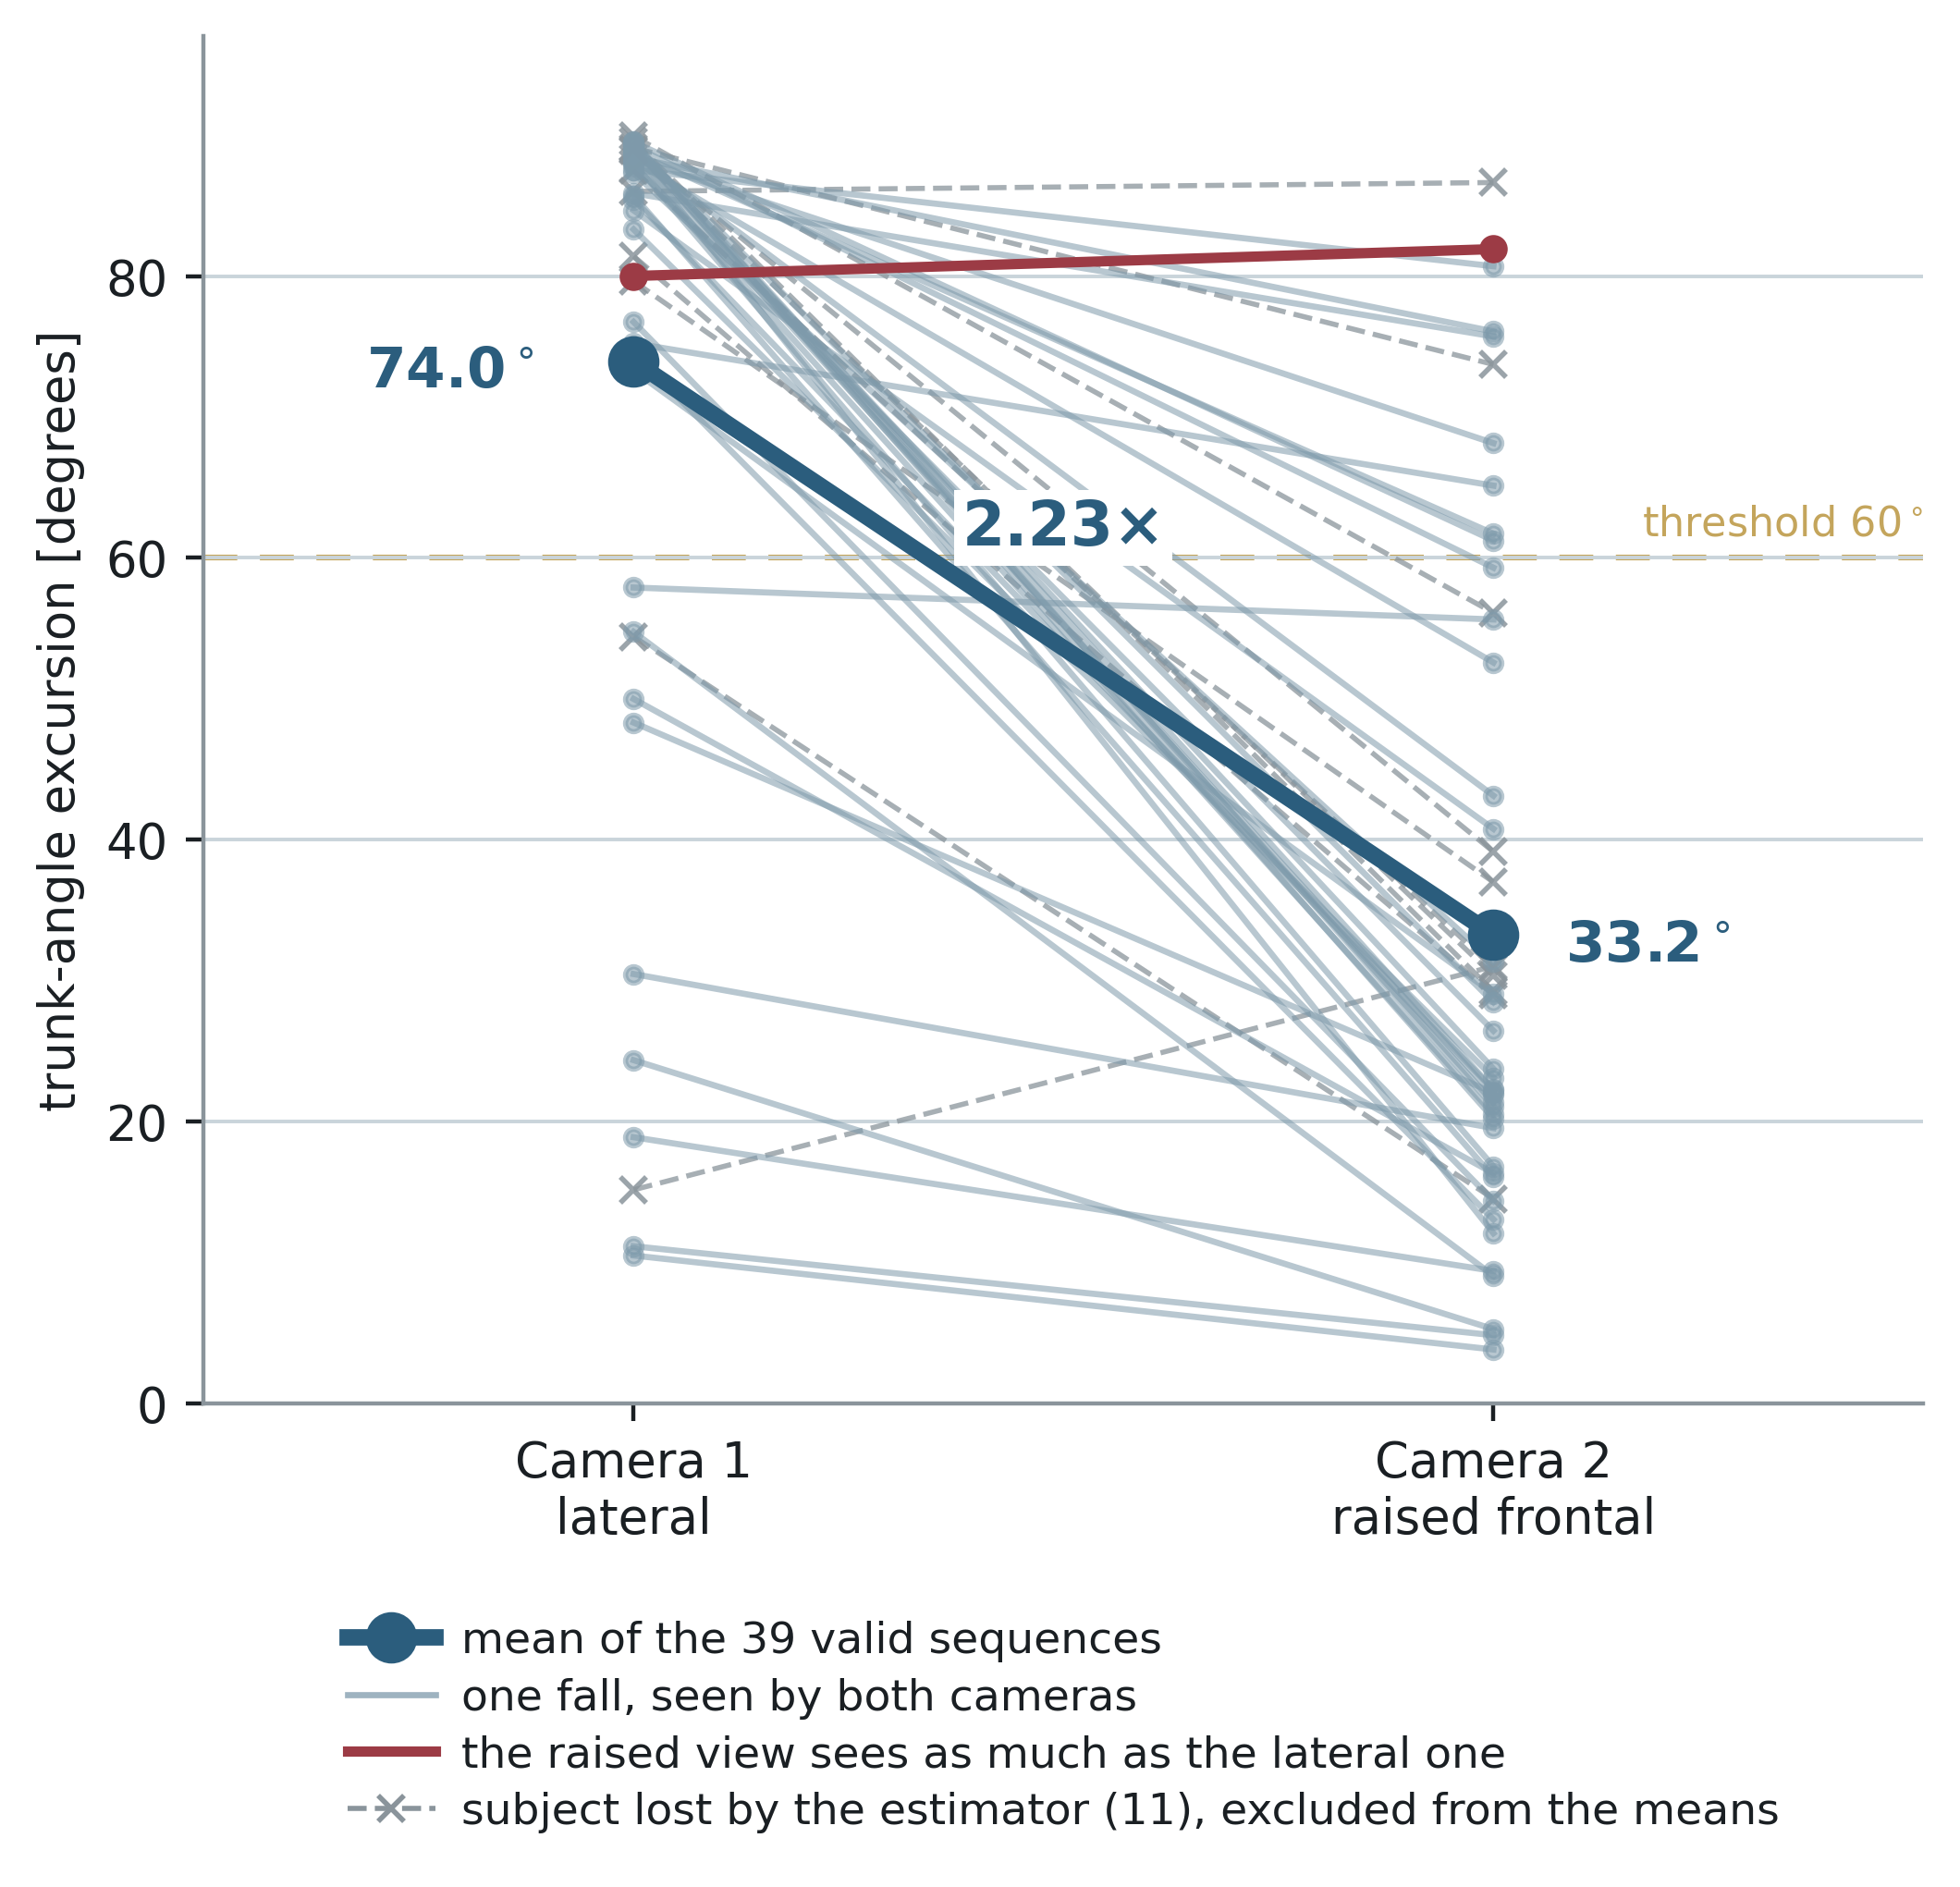
\includegraphics[width=\textwidth]{figure/fig_viewpoint_dist_en.png}
\caption{Excursion of the trunk angle in the two views for the 39 valid sequences.}
\label{fig:viewpoint_dist}
\end{figure}

The geometric difference also appears in the performance of the classifier.

\begin{table}[htbp]
\centering
\caption{Performance as the views used for training and test vary. Representation A3i (twelve quantities, without $h_{\text{pav}}$), random forest, three-class formulation, threshold $0{,}50$.}
\label{tab:viste}
\begin{tabular}{lccc}
\toprule
\textbf{Training} & \textbf{Test} & \textbf{$F_2$} &
\textbf{False positives} \\
\midrule
Camera 1 & Camera 1 & $0{,}822 \pm 0{,}099$ & 722 \\
Camera 1 & Camera 2 & $0{,}488 \pm 0{,}119$ & 3.252 \\
Camera 1 + Camera 2 & Camera 2 & $0{,}731 \pm 0{,}188$ & 751 \\
\midrule
Camera 2 & Camera 2 & $0{,}753 \pm 0{,}179$ & 1.067 \\
\bottomrule
\end{tabular}
\end{table}

\begin{figure}[htbp]
\centering
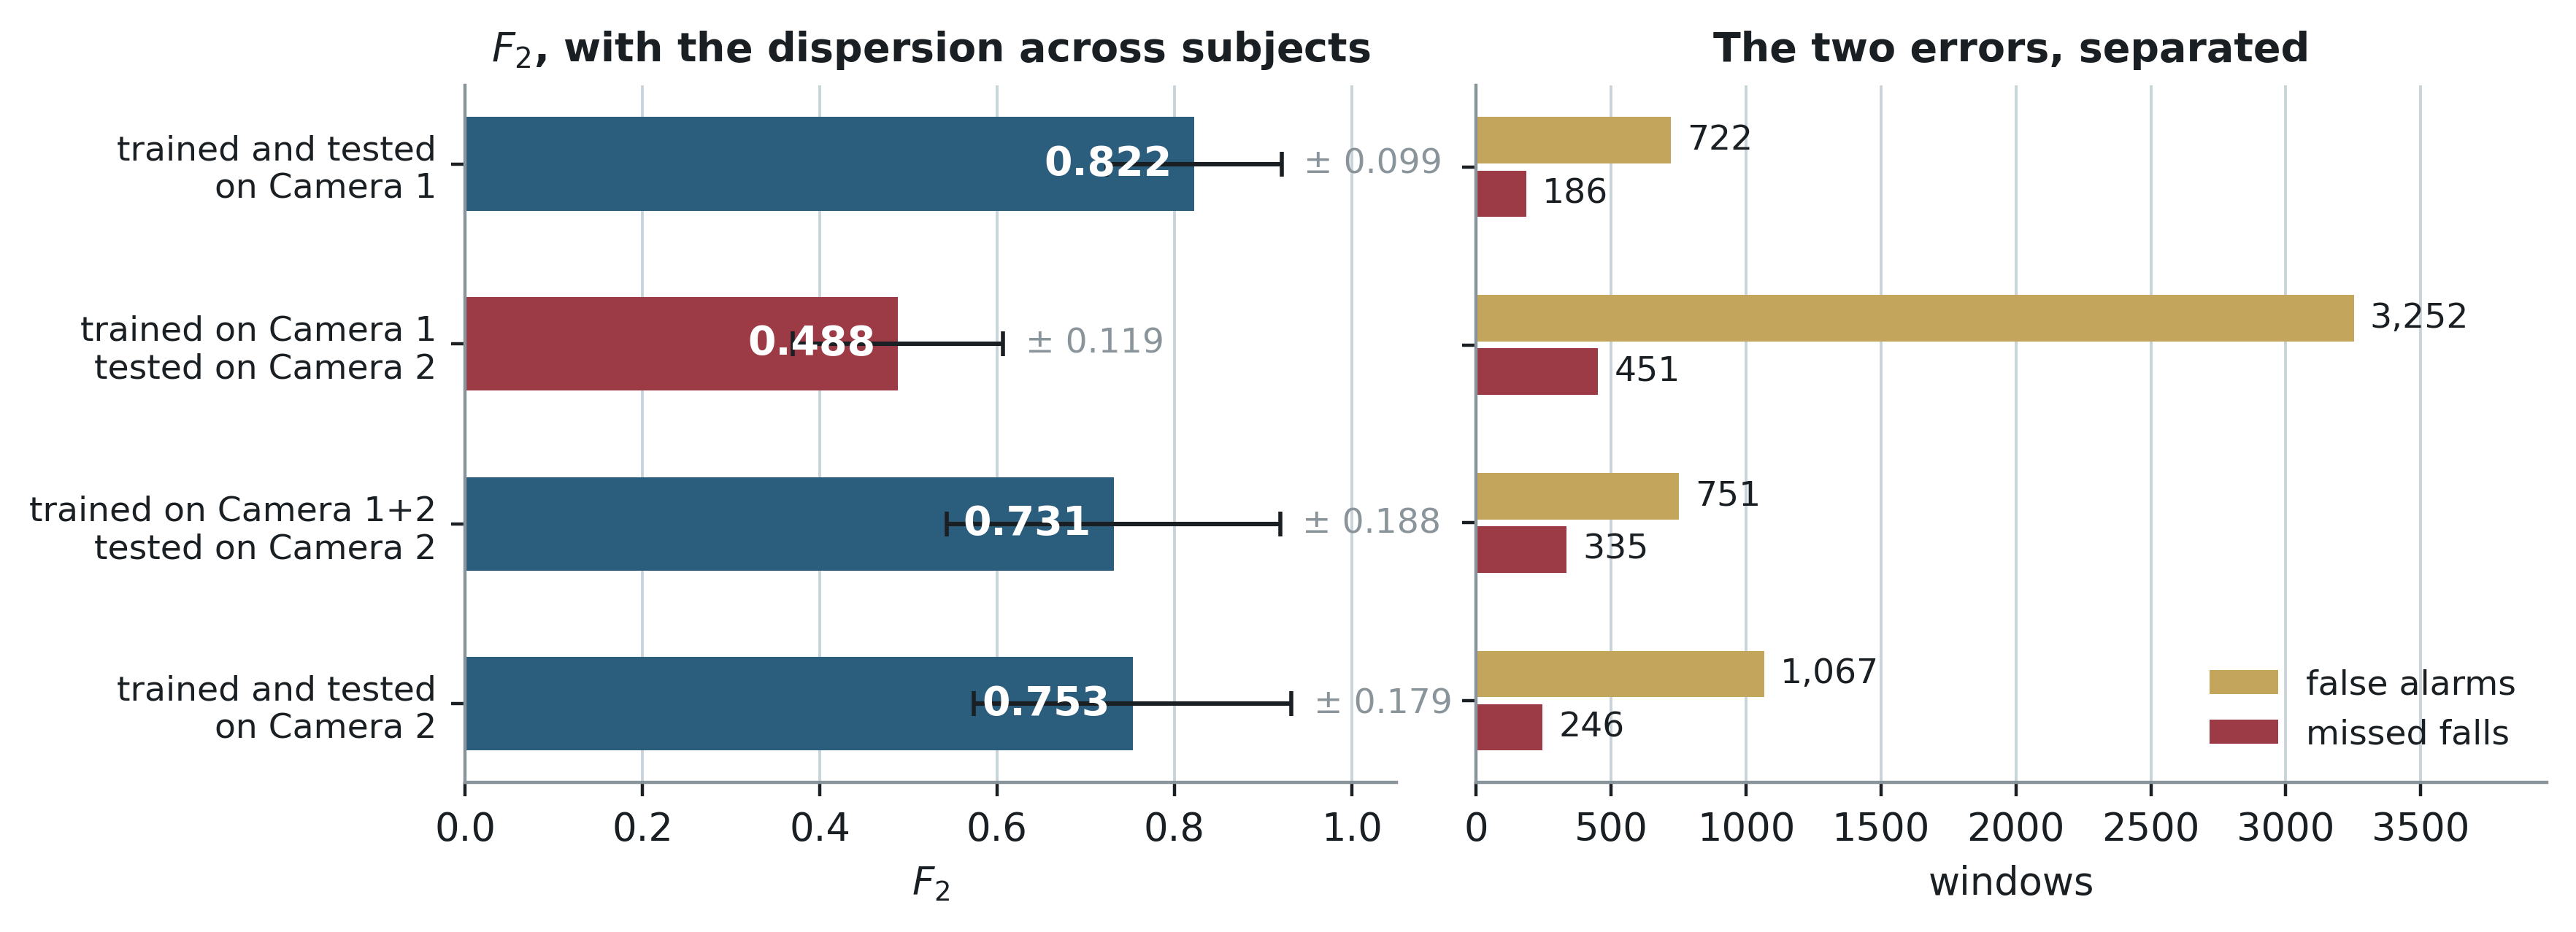
\includegraphics[width=\textwidth]{figure/fig_viste_en.png}
\caption{Performance obtained by changing the view used during training and test.}
\label{fig:viste}
\end{figure}

Training and evaluating the model on Camera~1 gives $F_2=0{,}822\pm0{,}099$. Applying the same model to Camera~2, the value drops to $0{,}488\pm0{,}119$, a loss of 0,334 of $F_2$, about three times the dispersion observed across subjects. The false positives rise at the same time from 722 to 3.252. When both views are included during training, on Camera~2 $F_2$ rises to 0,731 and the false positives fall to 751. Recall and precision also increase, from 0,670 to 0,762 and from 0,316 to 0,713 respectively.

The variability due to the viewpoint can therefore be reduced by including several geometries during training, but a difference with respect to the lateral view remains. An example is shown in Figure~\ref{fig:due_camere}.

\begin{figure}[htbp]
\centering
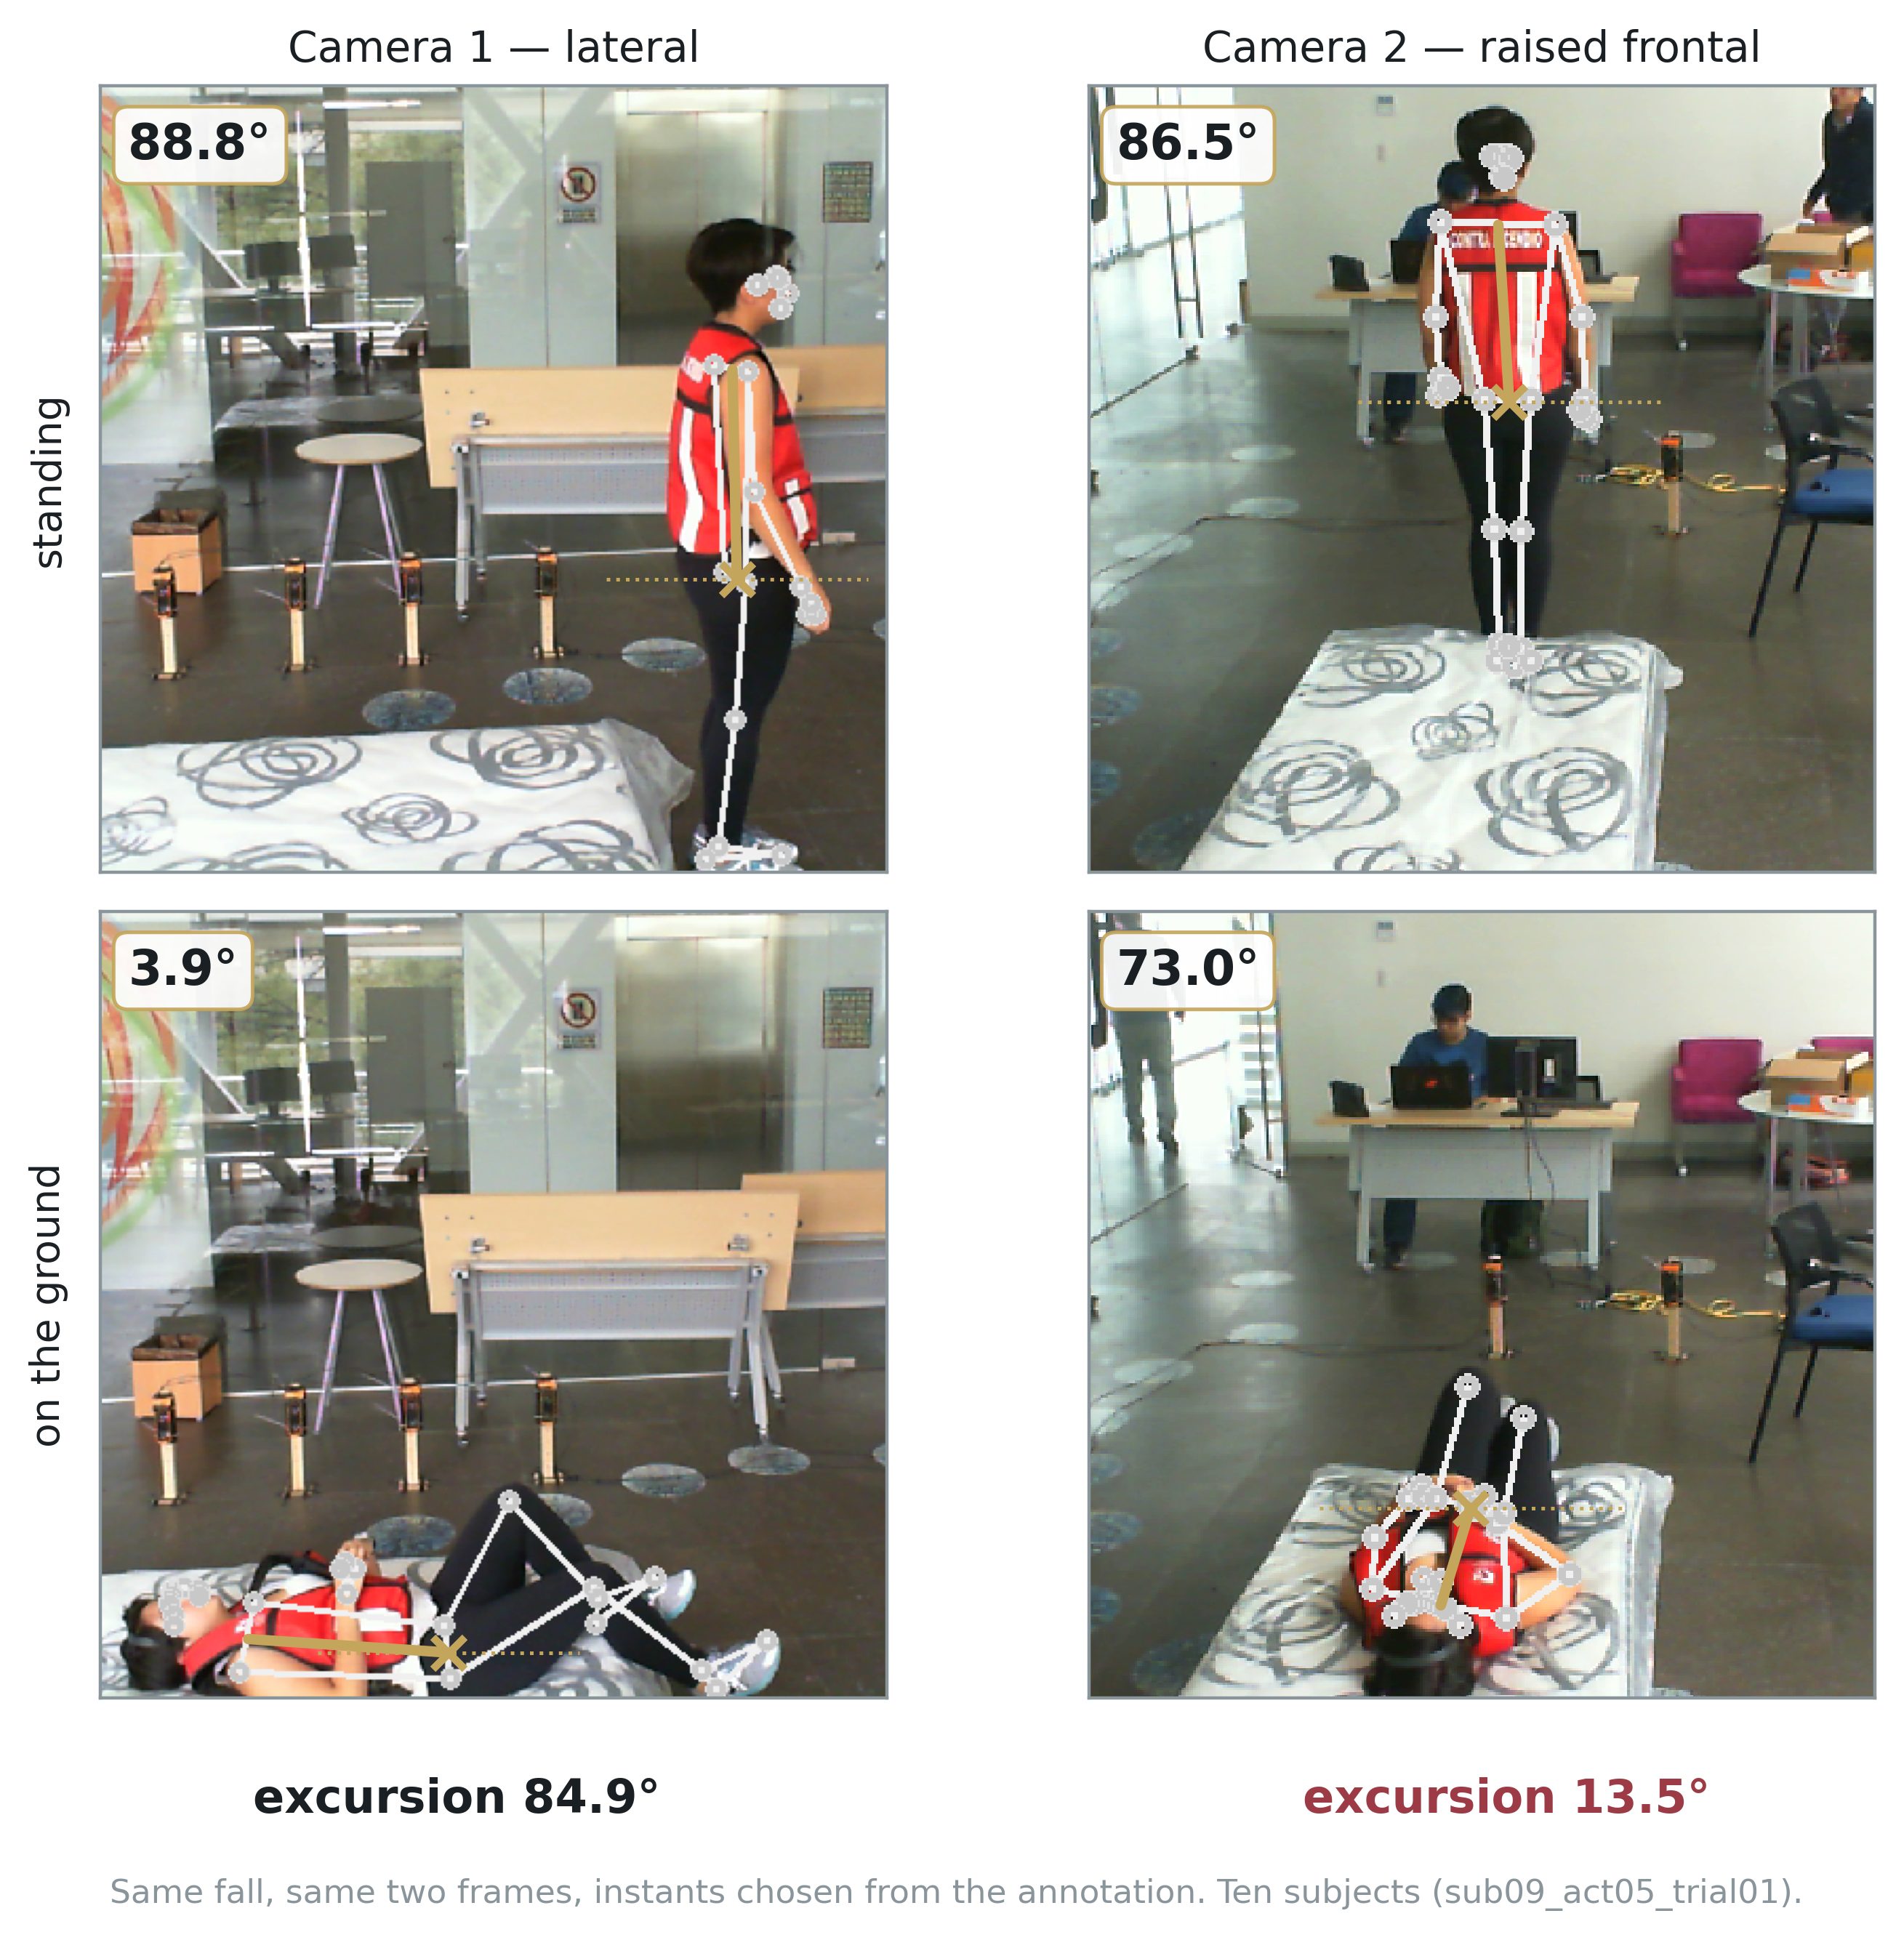
\includegraphics[width=0.85\textwidth]{figure/fig_due_camere_en.png}
\caption{The same fall observed from Camera~1 and from Camera~2. In the lateral view the excursion of the trunk angle is $84,9^\circ$, whereas in the raised frontal view it is $13,5^\circ$.}
\label{fig:due_camere}
\end{figure}

The geometry also changes $h_{\text{pav}}$. The separation between the medians of the two classes is $+1{,}510$ trunk lengths in the lateral view and only $+0{,}060$ in the raised frontal one. The feature therefore loses almost all its separating power when the camera is placed frontally and from above. This is why the criterion of Section~\ref{sec:dtw}, which
considers both cameras, does not include it in the main subset

\subsection{Transfer to an external dataset}
\label{sec:domainshift}

LOSO changes the subject but leaves dataset, environment and acquisition procedure unchanged. In order to assess the behaviour under conditions further from those of training, the model was also applied to UR-Fall, used as an external dataset. With respect to UP-Fall, the subjects, the environment and the recording modalities all change.

The annotations of the two datasets are not directly compatible. UP-Fall distinguishes the fall transition from the post-fall state, whereas UR-Fall describes mainly the posture. UR-Fall is therefore re-extracted with the same pose estimator and the same geometric engine, and the annotations are mapped onto the three phases used in the pipeline. The extraction comprises 11.400 frames distributed over 67 recordings and produces the same 33 candidate features.

The pose is available in 81,0\% of the frames, against 92,3\% for Camera~1 of UP-Fall. Two different trials were carried out on the external dataset. In the direct transfer, model and threshold are kept unchanged. In the diagnostic recalibration the model remains unchanged, while the threshold is recomputed using the labels of UR-Fall. The first experiment therefore measures the actual behaviour of the system on the new dataset. The second serves only to distinguish how much of the loss is due to the calibration of the threshold and how much to a reduction in discriminative power.

\subsubsection{Direct transfer}
\label{sec:esterno}
Since the prevalence of the positive class changes between the datasets, the PR-AUC was also considered, which measures the ability of the classifier to rank the positive windows irrespective of the threshold chosen. For a random classifier the expected PR-AUC coincides with the prevalence. We therefore define

\[
G_{\mathrm{PR}} = \frac{\mathrm{PR\text{-}AUC}} {\mathrm{prevalence}},
\]

Table~\ref{tab:esterno} reports the results obtained on UR-Fall.

\begin{table}[htbp]
\centering
\caption{Transfer from UP-Fall to UR-Fall.}
\label{tab:esterno}
\small
\begin{tabularx}{\textwidth}{@{}Xcccc@{}}
\toprule
\textbf{Configuration} &
\textbf{Prevalence} &
\textbf{PR-AUC} &
\textbf{Gain} &
\textbf{$F_2$ at $\theta=0{,}50$} \\
\midrule
A3 without integrals
& 0,130 & 0,440 & 3,4$\times$ & 0,404 \\
A3 with integrals & 0,130 & 0,466 & 3,6$\times$ & 0,479 \\
DTW subset & 0,130 & 0,660 & 5,1$\times$ & 0,630 \\
\midrule
Previous configuration
& 0,094 & 0,169 & 1,8$\times$ & 0,034 \\
\bottomrule
\end{tabularx}
\end{table}

Among the three directly comparable configurations, the ratio between PR-AUC and prevalence goes from 3,4 for A3 without integrals to 3,6 with the integral quantities, and reaches 5,1 with the subset selected by DTW.

The $F_2$ at the threshold fixed on UP-Fall also increases, from 0,404 to 0,479 and finally to 0,630. The DTW subset therefore retains a greater separating power on the external dataset than the other two configurations, while still showing a degradation with respect to the training domain. The previous configuration uses a different definition of the positive and a prevalence of 0,094. Its gain is therefore not directly comparable with the other three and is reported as a point of reference.

\begin{figure}[htbp]
\centering
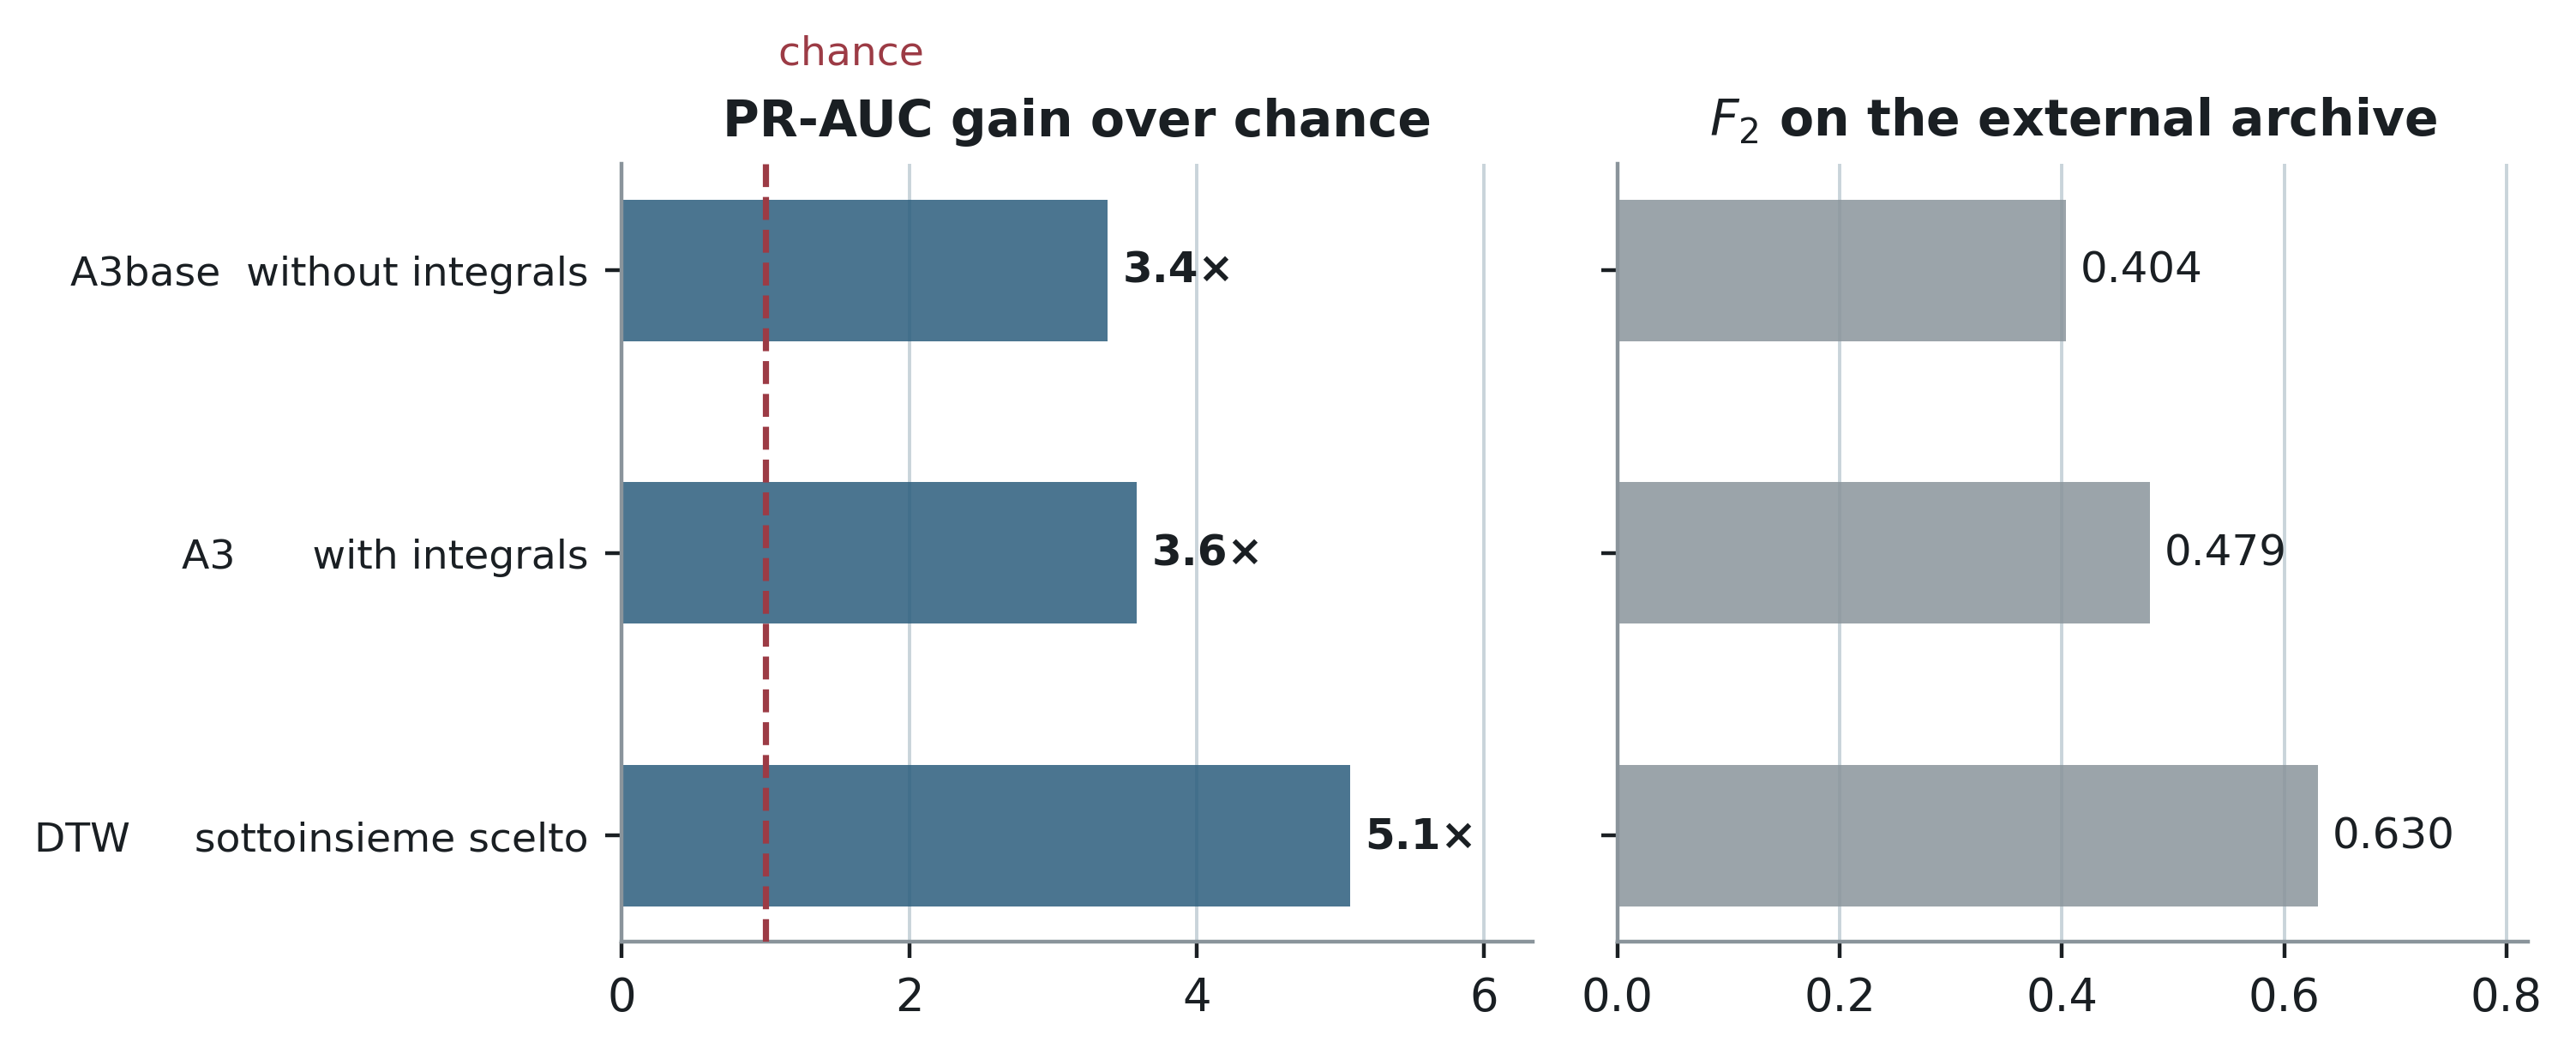
\includegraphics[width=0.85\textwidth]{figure/fig_esterno_en.png}
\caption{Performance in the transfer to UR-Fall. On the left the ratio between PR-AUC and prevalence is reported, while on the right the $F_2$ obtained with the threshold fixed on the source dataset is shown.}
\label{fig:esterno}
\end{figure}

\subsubsection{Diagnostic recalibration}

The degradation on an external dataset may depend on two different phenomena. The first is a loss of calibration: the model retains part of its ability to rank the windows, but produces scores on a different scale. The second is a loss of discriminative power: the two classes become harder to separate. In order to distinguish the two effects, a second trial was carried out on the previous configuration, recomputing the threshold that maximises $F_2$ directly on UR-Fall.

This threshold uses the labels of the target dataset and is therefore called the \emph{oracle threshold}. It does not represent a procedure usable in a real installation, because it requires knowing in advance the labels of the data to which the system is to be applied.

\begin{figure}[htbp]
\centering
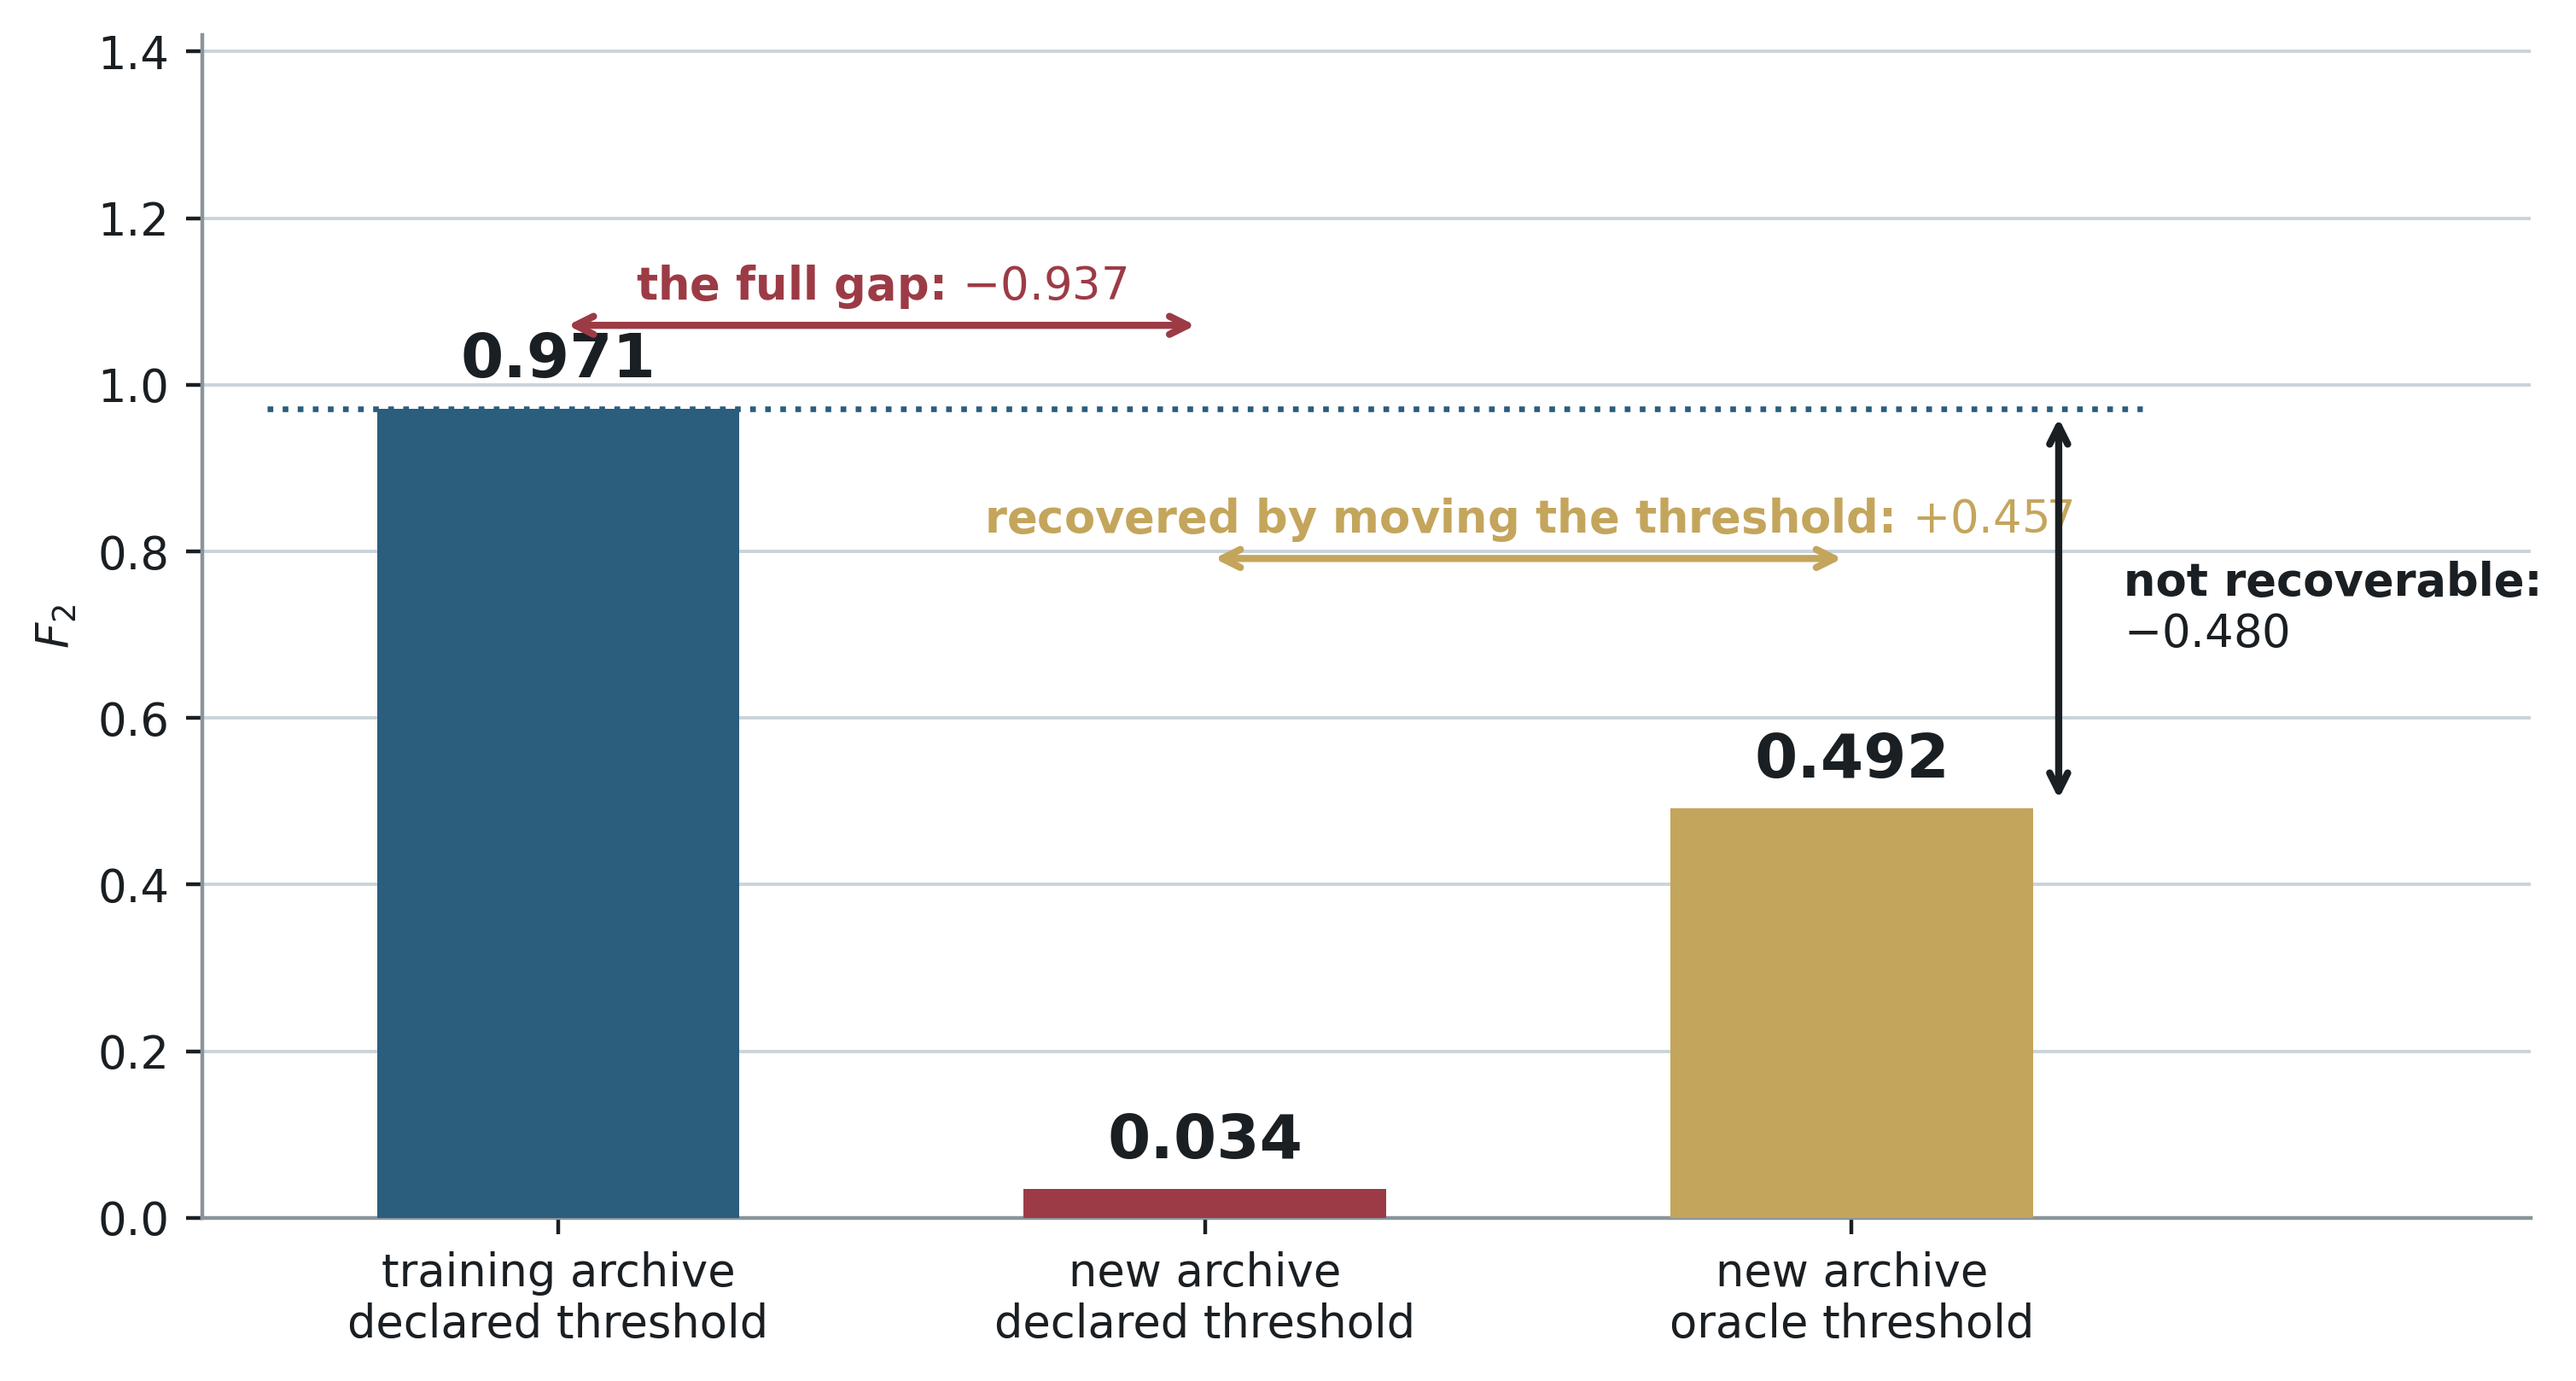
\includegraphics[width=0.85\textwidth]{figure/fig_dominio_en.png}
\caption{Decomposition of the gap between the source domain and UR-Fall into loss of calibration and loss of discriminative power.}
\label{fig:dominio}
\end{figure}

With the threshold fixed on UP-Fall, the previous configuration obtains $F_2=0,034$ on UR-Fall. With the oracle threshold the value rises to 0,492. In the source domain the same configuration reached about 0,971. Of the 0,937 points of difference, about 0,457 are recovered by changing the threshold, while about 0,480 remain even after recalibration.

The drop therefore does not depend on the threshold alone. Even after the decision point has been adapted, a substantial loss of discriminative power remains. The same conclusion is consistent with the PR-AUC: in the previous configuration the ratio with respect to the prevalence goes from about 18,7 in the source domain to 1,79 on UR-Fall. This decomposition was carried out only on the previous configuration and must not be attributed directly to the DTW subset. For the latter the direct transfer is available, with a PR-AUC of 0,660 and $F_2=0{,}630$ at the threshold fixed at 0,50.

A loss of calibration can be addressed by changing the decision
threshold, whereas a loss of discriminative power requires
intervening on the model or on the data used to train it. Supervised recalibration would in any case require labelled examples from the new environment, which are not normally available at the time of installation. The oracle threshold is therefore used only as a diagnostic tool and not as a level of performance actually achievable by the system on the external dataset.
